\documentclass[a4paper,onecolumn]{article}
\usepackage{amsmath, amsthm, graphicx, amssymb, wrapfig, fullpage, subfigure, array,float}
\usepackage[]{algorithm2e}
\usepackage[toc, page]{appendix}
\usepackage{pdfpages}
\usepackage{tikz}
\usetikzlibrary{positioning,shadows,arrows}
\usepackage[font=sl, labelfont={sf}, margin=1cm]{caption}
\DeclareMathOperator{\e}{e}
\newtheorem{definition}{Definition}
\theoremstyle{remark}
\newtheorem{theorem}{Theorem}
\newtheorem{remarker}{Remark}

\begin{document}
\setcounter{page}{1}
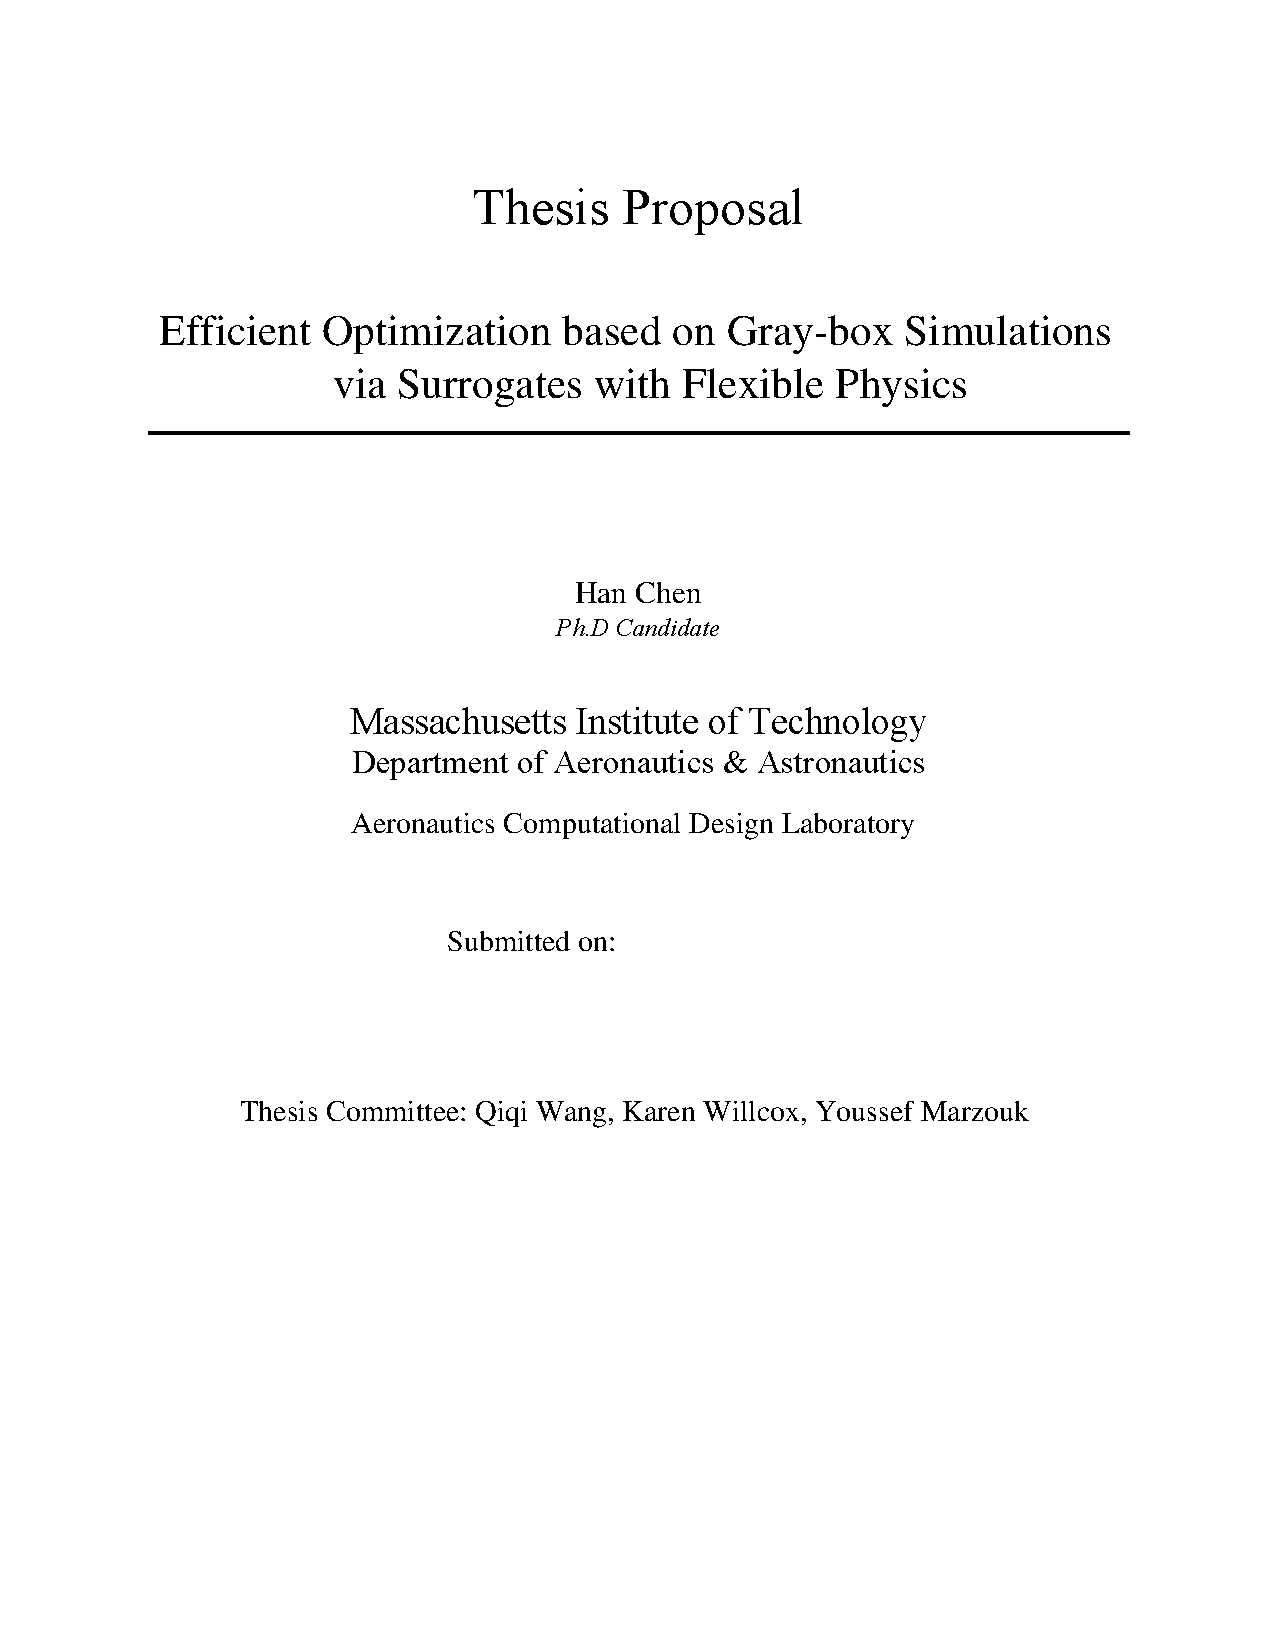
\includepdf[pages=-]{cover}
$$ $$
\newpage
\tableofcontents
\newpage
\section{Background}
\label{intro}

\subsection{Optimization based on gray-box PDE simulation}
Optimization problems is of great interest in the engineering community. We consider minimizaing an
objective function:
$$
    J: \mathcal{C} \in \mathbb{R}^d\times [0,T] \rightarrow \mathbb{R}, \qquad c(t) \rightarrow J(c)\,,
$$
where $c(t) \in \mathbb{R}^d$ for $\forall t$. $c(t)$ is the control variable to be optimized.
In many cases, the objective function is an ouput of
a PDE based, spatial-time simulation. 
These simulations are generally implementations of physics models, and can provide accurate predictions for
the output quantity of interest.
For illustration purpose, we will mostly use oil reservoir management and optimization problems.
Though the method being developed is not restricted to reservoir problems.\\

\noindent In many cases, PDE-based simulations implement complex physics models and exotic solution techniques, and
the physics models and implementations of solving the PDEs may not
be accessible. For example, many industrial reservoir simulators are proprietary, such as \textit{Eclipse} (Schlumberger), 
\textit{VIP} (Halliburton), and \textit{PSim} (ConocoPhillips). During an internship in ConocoPhillips, the author got a chance to
look at \textit{PSim}'s source code. It turns out to be a million-line, \textit{Fortran77}, legacy code developed for decades.
Therefore, even when the source code and the documentation are availble, it can still take tremendous amount of man power
to access or modify the code.
We call such simulations \emph{black-box}, in the sense that the only duty of the simulation is to compute the objective function:
\begin{equation}
    J = J(c;\kappa) \in \mathbb{R}\,,
\end{equation}
where $\kappa\in \mathbb{R}^n$ are some pre-defined model properties (for example, porosity and permeability in oil reservoir simulation).
$c$ is the control variable to be optimized. The controls can also be not inside the PDE,
but are parameters that defines the spatial domain of solving the PDE, for example, 
in airfoil optimizations.
Fortunately, although it may be difficult to access the details of the simulation, it's 
often easy to write down
the abstract form of the PDE. For example, many reservoir simulations can be written as \cite{reservoir simulation book}
\begin{equation}\begin{split}
    &\eta\frac{\partial u}{\partial t} + \nabla \cdot F(u, \kappa) = q(u,c)\\
    &J = \int_0^T\int_\Omega j(u,c) \; \textrm{d}t \textrm{d}\mathbf{x}
\end{split}\end{equation}
generally with an impermeable boundary condition or other known boundary conditions. 
$u\in \mathbb{R}^n$ includes field quantities like pressure and saturation. $\eta, \kappa\in \mathbb{R}^n$ 
are geology properties like porosity and permeability. $q\in \mathbb{R}^n$ is a known or
unknown model for the volumetric change of $u$. 
$F\in \mathbb{R}^n$ is an unknown flux term. And $c$ is the time-space-dependent control variable, for example 
water injection rates. Another observation is, 
given $c$ and $\kappa$, many simulators can output the discretized $u(t,x)$ in addition to $J$.
We will call such simulations \textit{gray-box} simulations \cite{review of black-box modeling}
, in order to distinguish \textit{black-box} simulations where 
the underlying PDE, the boundary conditions, and $u(t,x)$ are unknown.
The opposite of black-box simulation is \emph{open-box} simulation.\\

\noindent Thanks to the complexity of physics models and large time-space scale involved, 
running a PDE-based simulation can be computationally expensive. 
In addition, optimization problems may entail a large number of 
PDE simulations. To give insights to this issue, let's suppose the time domain $[0,T]$ is discretized into $m$ points, 
then we need to search in a $\mathbb{R}^{d\times m}$
space for the optimum. When $d\times m$ is larger, more simulations may be invoked due to the larger search space.
Therefore optimization based on PDE-simulations can be costly.\\

\noindent We will restrict our attention to optimization based on gray-box simulations with a high-dimensional control space.

\subsection{Problem setup}
\label{psetup}
We consider the PDE governing the gray-box simulation to take the form:
\begin{equation}
    \frac{\partial\eta_i u_i(t,x)}{\partial t} + \nabla \cdot 
    F_i(\mathcal{D} u, \kappa) 
    = q_i(u,c(t,x))\,, \qquad i=1,\cdots, n\,,
    \label{first equation}
\end{equation}
where $x\in \Omega \subseteq \mathbb{R}^{n}$ is the spatial coordinate.
$\partial \Omega$ is the boundary. $t\in[0,T]$ is time.
The boundary condition is known. $F_i(\cdot, \cdot)$'s are the unknown flux functions. 
$u = \{u_1, \cdots, u_n\}$.\\
$\mathcal{D} u = \left\{u_1, \nabla u_1 , \cdots, \nabla^{i_1} u_1; \cdots;
u_n, \nabla u_n,\cdots, \nabla^{i_n} u_n\right\}$, where $\nabla^j$ indicates the $j$th
order spatial derivative tensor. We assume $i_1,\cdots, i_n$, i.e. the maximum 
order of derivatives, are known.
$\eta_i=\eta_i(x), \,\kappa=\kappa(x)$ are 
problem dependent spatial variables, and is assumed known. $c(t,x)$ is a spatial-time-dependent control variable.
$q_i(\cdot,\cdot)$'s are known or unknown functions.
The discretized space-time solution of Eqn\eqref{first equation} given by a simulator
is written as $\hat{u}(t_i, \mathbf{x}_i; c)\,,\, i=1,\cdots,N$.\\

\noindent The objective function is defined by
\begin{equation}
    J = \int_0^T \int_\Omega j(u,c) \textrm{d}\mathbf{x}\textrm{d}t
\end{equation}
Notice $j$ can depend explicitly on c, while $u$ depends implicitly on $c$.\\

\noindent Let's consider a concrete example. Consider a simulator modeling two phase flow in porous media.
One of the simplest yet classical model for two-phase porous media flow is the Buckley-Leverett model \cite{Buckley Leverett}. 
It models the displacement process of two-phase flow due to capillary pressure and Darcy's law \cite{Reservoir Simulation Book}.
The PDE, Buckley-Leverett equation, is
\begin{equation}
     \frac{\partial u}{\partial t} + \frac{\partial}{\partial x} \left(\frac{u^2}{1+A(1-u)^2}\right) = c\,,
\end{equation}
where $u = u(t,x)$, $0\le u\le 1$, is the saturation of phase I (e.g. water), and $1-u$ is the saturation of
phase II (e.g. oil). $A>0$ is a parameter dependent on the physical property of the two phases.
$c=c(t,x)$ is the control variable. $c>0$ models the injection of phase I replacing phase II; and $c<0$ vice versa.\\

\noindent Suppose we want to control the flow through $c$, such that the saturation at $t=T$ is close to 
a target saturation $u^*(x)$. We introduce an $L_2$ penalty to the objective function for regularization \cite{Boyd optimization}.
The regularization can be interpreted as the cost of control. Hereby the objective function
\begin{equation}\begin{split}
    J &= \int_x \left|u(T,x) - u^*(x)\right|^2 \textrm{d}x + \eta \int_t\int_x  c^2(t,x) \textrm{d}x\textrm{d}t\\
      &= \int_t \int_x \left|u(t,x) - u^*(x)\right|^2 \delta_T(t) + \eta c^2(t,x) \textrm{d}x \textrm{d}t \,,
\end{split}\end{equation}
where $\eta>0$ models the magnitude of the regularization, and $\delta_\cdot(\cdot)$ indicates the Direc delta function.
The optimization problem is
\begin{equation}
    c^* = \arg\min_{c\in \mathcal{C}} J
\end{equation}
where $\mathcal{C}$ is the $L_2$-function Hilbert space. Notice the optimization is unconstraint.\\

\subsection{Gradient-free and gradient-based optimization}
\label{gradfree_gradbased}
\noindent Existing methods for optimization can be classed into two categories: 
using gradient information (gradient-based optimization) and not using gradient information (gradient-free optimization)
\cite{hanmaster, Opt Koziel Book}.
Gradient-free optimization methods require only the availability of objective function values but
not derivative information\cite{gradfreereview}. Because of its mild requirement of the simulation, 
gradient-free optimization methods are suitable for optimization problems based
on \textit{black-box} simulations, and enjoy a wide range of applicability. However, when the dimension of the search space 
$d\times m$ increases, these methods generally suffer from the \textit{curse of dimensionality}.
The term \textit{curse of dimensionality} refers to problems caused by the rapid increase in the search volume associated
with adding extra dimension in the search space\cite{dynamicprogramming}. It's not uncommon to encounter
hundreds of dimensions in real life engineering problems, limiting the applicability of gradient-free optimization
in these cases.
Several strategies have been proposed to address this challenge
\cite{survey of high dimensional blackbox optimization}, such as
dimensional reduction \cite{dimensional reduction}, system decomposition \cite{decomposition},
and variable selection \cite{variable selection}. However, these methods generally assumes
special structures of the system to work properly \cite{survey of high dimensional blackbox 
optimization}.\\

\noindent In contrast, gradient-based optimizations use gradient information to locate the local optimum.
A well-known example is the quasi Newton's methods \cite{quasiNewton}. 
Generally gradient-based methods require less number of simulations 
to converge than gradient-free methods, and are more efficient at finding local optimum for high-dimensional problems.
In addition of requiring $J(c)$ from the simulation,
these methods also require $\frac{\partial J}{\partial c}$, the sensitivity.
Adjoint methods are efficient methods for sensitivity analysis\cite{cont discretize adjoint}
for open-box models.
Continuous adjoint method develops the continuous adjoint equations from the continuous PDE of the simulation through 
Lagrange multiplier; and it requires the PDE of the simulation. 
Discrete adjoint methods applys variational methods directly to the discretized PDE; and it requires the
discretized PDE (i.e. the numerical implementation) of the simulation. Thus, adjoint methods can not be applied
to compute the sensitivity of a black-box simulation.
Another popular method to compute sensitivity is automatic differentiation (AD)\cite{automaticdiff}.
AD exploits the fact that every computer program can be broken down into a sequence of elementary arithmetic operations
and elementary functions. By applying the chain rule repeatedly to these operations, 
derivatives of arbitrary order can be computed automatically. Because AD requires the accessibility of every elementary 
operation during a simulation, it can not be used to compute the sensitivity of a black-box simulation either.\\

\noindent To sum up, gradient-free optimization methods are suitable for gray-box simulations, but suffer from the curse of
dimensionality; gradient-based optimization methods are more efficient for high-dimensional problems, but are not suitable for 
gray-box simulation. This dilemma motivates the development of a new optimization strategy. 
The objective of my thesis is to design a new optimization strategy that: 1. not require $\frac{dJ}{dc}$ from the gray-box simulation, and 2. be suitable for high-dimensional 
problems.\\

\subsection{Proposal outline}
\noindent In the following chapters we will develop a new optimization strategy to address this
problem. 
The first step of the new strategy is to construct a surrogate of $\frac{dJ}{dc}$ 
(gradient surrogate) using only the input and output of the
gray-box simulation. We will develop such a surrogate in section \ref{gradient_surrogate} and section \ref{adaptive}:
section \ref{gradient_surrogate} discusses the surrogate with fixed structure; whereas section \ref{adaptive} discusses the surrogate
with an adaptive structure. The next step of the strategy is to optimize $J(c)$ using both the
samplings of $J(c)$ and the samplings of the gradient surrogate.
In section \ref{bayesian_model} we will model the objective function and the surrogate as
realizations of stochastic processes, hereby
unify the samplings of $J(c)$ and the gradient surrogate inside a Bayesian framework. In section \ref{bayesian_opt} we will apply an Bayesian optimization method, 
the expected improvement algorithm \cite{jones1998},
to the unified Bayesian modelling, and discuss its convergence. In section \ref{complete_algo} we will summarize the algorithm. A numerical example of water-oil displacement process will be shown in chapter \ref{examples} to illustrate the advantage of the new strategy.\\

\newpage
\section{Twin model}
\label{gradient_surrogate}
\subsection{Review of surrogate methods}
\label{review surrogate methods}
\noindent As mentioned in chapter \ref{intro}, 
straightforward optimization of the objective function, i.e. by applying
optimization routine directly to $J(c)$, is not always practical.
A well-studied topic to address this problem is \emph{surrogate-based optimization}
\cite{Opt Koziel Book, Surrogate based analysis and optimization}.
It is proposed to achieve optimization at reduced computational cost \cite{Space mapping 1}.
A \emph{surrogate} is a reasonably accurate representation of the high-fidelity model $J(c)$.
In the following context we will call the high-fidelity $J(c)$ the \emph{primal model},
and write the surrogate model as $\tilde{J}(c)$.
In surrogate-based optimization, the optimization of the primal model is
replaced by iteratively updating and re-optimizing the surrogate.
The design point generated by optimizing the surrogate is verified by evaluating
the primal model. The primal model evaluation is then used to update the surrogate.
Surrogate-based optimization generally proceeds in this prediction-correction manner until
termination.\\

\noindent Surrogate-based optimization methods can be distinguished by how the surrogate is 
constructed. Surrogate construction techniques can be categorized into
\emph{physics-based surrogate} and \emph{functional surrogate} \cite{Opt Koziel Book}.
Similar to the primal model, physics-based surrogate simulates the underlying physics.
The surrogate is still a representation of the underlying system's physics, but has 
lower fidelity and is cheaper to evaluate: generally because it
uses simplified physics \cite{simplified physics, Space mapping 1} and/or
uses coarse discretization \cite{coarse discretization}.
A functional surrogate, on the other hand, are constructed using only the sample
values of $J(c)$ obtained from the primal model (and gradient of $J(c)$ if
the primal model can also evaluate the gradient \cite{gradient kriging surrogate}).
Functional surrogate does not require previous knowledge of the physics system of interest. 
Popular functional surrogate techniques include polynomial approximation 
\cite{poly functional surrogate}, Kriging \cite{kriging functional surrogate},
and artificial neural network \cite{ann functional surrogate}, etc.\\

\noindent Generally, physics-based surrogates are more expensive to evaluate but more accurate,
mainly because they already embed some knowledge of the system's physics. 
However, physics-based surrogates are dedicated to the specific systems of interest.
The construction of physics-based surrogates often require expert insights
and significant coding manpower \cite{Opt Koziel Book}. 
Functional surrogates, on the other hand, are generic to a wide class of problems.
The price paid is they may require considerable amount of primal model evaluation 
to achieve the same accuracy as physics-based surrogates. \\

\noindent Designing a good physics-based surrogate requires expert insight
(e.g. the choice of empirical formulas or the negligence of unimportant physics components),
thus limits its applicability. Another drawback lies in the fact their underlying
physics is fixed. Generally these models are only good approximation of the primal model
within a certain range of physics settings. In optimization, however, design parameters 
move at each iteration. A low-fidelity model may gradually lose its accuracy 
as the design parameters moves away from the surrogate's applicable region.
For example, the thin airfoil theory is only valid before stall. 
If one is to optimize the attack angle, the thin airfoil models may no longer 
provide good estimation of the primal model when the attack angle increases \cite{thin airfoil}.
Another example is from turbulent modelling.
Some simplified fluid models are derived under the assumption of low Reynolds number
\cite{turbulent modeling R low}, while some are derived under high Reynolds number 
\cite{turbulent modeling R high}.
If one is to optimize the flow speed, the quality of using the simplified fluid models
as surrogate can be questionable.\\

\noindent To sum up, physics-based surrogates have two drawbacks:
1. They require expert knowledge for construction. 2. Their physics are fixed offline
and may not always give good approximations during optimization.\\

\subsection{Envision of twin model}
\noindent To alleviate these drawbacks, we can \emph{correct} the surrogate's objective function
iteratively online to improve its accuracy. 
One method is \emph{Bayesian model calibration}
\cite{KennedyOhagan1, andrewras}. This approach models the (global) error,
$J(c) - \tilde{J}(c)$, as a deterministic but unknown  
realization of a stochastic process. 
Hereby infer the error at unsampled $c$ via a Bayesian framework,
using existing samples of $J(c)$ and $\tilde{J}(c)$.
The inferred error is then added to $\tilde{J}(c)$ to provide a corrected surrogate.
Another method is \emph{multi-fidelity trust-region method}, i.e. to bound the search step
inside a \emph{trust region} during each optimization iteration \cite{trustregionwild}.
Within each trust region, the surrogate can be corrected to guarantee good (local) estimation
of the primal model (e.g. satisfying the \emph{fully-linear} property \cite{trustregionconn}),
thus guaranteeing convergence.\\

\noindent These research efforts (Bayesian model calibration, multi-fidelity 
trust-region methods, etc) can be viewed as overlaying the existing surrogate model with 
an additional \emph{functional}
surrogate for correction. In order for the correction to improve the existing surrogate 
to a desirable accuracy, a large number of primal model evaluations may be required.
As we mentioned earlier, this is a common problem suffered by functional surrogate.
In the mean time, the \emph{physics} of the physics-based surrogate is still fixed offline
before the optimization. Can we use primal model samplings to
directly correct the physics of the surrogate? Bearing this question at mind,
we propose \emph{twin model}: a physics-based surrogate model with flexible physics.\\

\noindent My envision is: the physics of twin model should have a learning
ability. In other words, twin model should be able to morph its representation of the 
underlying system's physics on-the-fly, so as to mimic the behavior of the primal model for
a wider range of physics settings.
Besides, according to our gray-box assumptions in chapter \ref{intro},
the learning process should treat the primal model non-intrusively.
In other words, the only knowledges available in the learning process
are sampled $J(c)$'s and corresponding space-time solutions $u(t,x;c)$'s of the primal model.
Finally, the learning process should be disciplined and automated. 
Once the optimization started, no human intervention would be required
to adjust the physics of the twin model.\\

\noindent Is the envision feasible? Consider a general dynamical system
\begin{equation}
    \dot{u} = \mathcal{L}(u)\,,
    \label{general equation}
\end{equation}
where $u=\{u_1,\cdots, u_n\}$, $u_i = u_i(t,x)$, $i=1,\cdots,n$, $x\in \mathbb{R}^n$.
$\mathcal{L}$ is a differential operator known as the Hamiltonian of the system 
\cite{Hamilton Fluid Dynamics}.
Suppose an observer can take snapshots of $u$ at any $t$.
It has been shown that inferring $\mathcal{L}$ from the snapshots is an intractable
problem, no matter how many snapshots are observed \cite{NP hard}.
Although Eqn\eqref{general equation} offers the most general description of the 
primal model, we may not be able to construct a practical twin model 
just based on Eqn\eqref{general equation}.\\

\noindent However, inferring the differential operator $\mathcal{L}$ 
is not necessary. As discussed in
chapter \ref{intro}, the PDE that governs the primal model 
can already be written as Eqn\eqref{first equation}. 
Therefore, the problem of adjusting twin model's physics reduces to the
problem of adjusting a set of functionals $F_i(\mathcal{D}u, \kappa)$, for 
$i=1,\cdots,n$. In addition, we can use the discretized space-time solution 
$\hat{u}(t_i,\mathbf{x}_i;c)$, provided by the primal model, to adjust the 
physics of twin model.
$\hat{u}(t_i,\mathbf{x}_i;c)$ is a by-product of evaluating $J(c)$,
but provides more information than $J(c)$ about the underlying system's physics
\cite{hanmaster}.
Finally, as we write the twin model in a conservative form, 
the implementation of twin model can be guaranteed to conform to conservation laws
using appropriate numerical schemes such as finite volume methods
\cite{numerical schemes for hyperbolic equation review}.\\

\noindent To sum up, we aim at inferring the functional $F_i$'s in Eqn\eqref{first equation}
using the space-time solutions $\hat{u}$ of the primal model.\\

\subsection{Review of system identification}
\label{SI review}
\noindent The inference problem is a \emph{system identification} problem. System identification is
a method that builds mathematical models of a
dynamical system from its measured data \cite{SI old}.
Depending on the how the system is modelled, system identification 
can be classified into \emph{linear system identification} and
\emph{nonlinear system identification}. Linear system identification assumes a linear
relationship between the system inputs $\mathbf{x}(t)$ and output $y(t)$:
\begin{equation}
    y(t) = h_0 + \sum_{i=1}^n \int_0^t h_i(\tau) x_i(t-\tau) \, d\tau
    \label{linear dynamic}
\end{equation}
The advantage is a linear model can be determined solely by its
impulse response function.
Clearly, the twin model
is generally nonlinear and may not be modelled well by a linear system.
Nonlinear system identification does not assume this linearity, thus is more generic
\cite{NARMAXbook}.
We will restrict our attention to nonlinear system identification.\\

\noindent Well-known models for nonlinear system identification include
\cite{NARMAXbook}: \emph{piecewise linear models},
\emph{block-structured models}, 
\emph{Volterra models}, and \emph{NARMAX} models. 
A piecewise linear model develops a series of locally linear approximations
to the system. In our problem, this model would adopt a piecewise linear 
representation of $F_i$'s and $q_i$'s. 
This approach can utilize the wealth of knowledge obtained from the research in linear systems.
But a drawback is the difficulty to partition the parameter domain, because
the estimation of piecewise model can not be easily separated from the task of finding the
domain for each sub-model \cite{piecewise linear}.\\

\noindent Block-structured models are described by connections of groups of linear 
and nonlinear models \cite{NARMAXbook}.
For example, Hammerstein model applies a nonlinear scaling of the input before transmitting
it to a linear dynamic model described by Eqn\eqref{linear dynamic}.
Wienner model, on the other hand, applies the nonlinear scaling after the dynamic model.
\begin{figure}[H]\begin{center}
    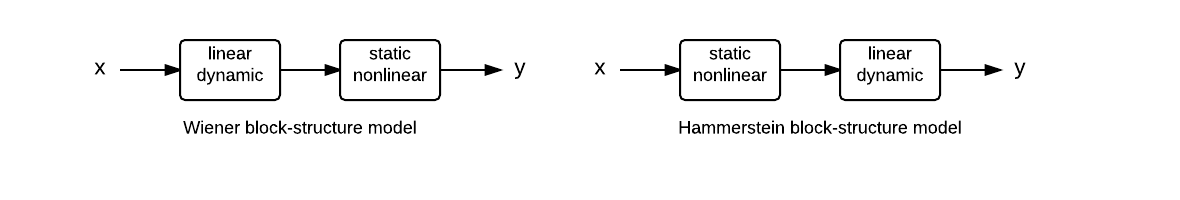
\includegraphics[height=2.5cm]{blockstructure.png}
    \caption{block structure model}
\end{center} \label{Wiener}
\end{figure}
\vspace{-.5cm}
\noindent 
These models became popular after theoretical results showing a nonlinear scaling operation 
preserves the cross variance of Gaussian stochastic signals \cite{cross correlation}. 
Another type of block-structured models are feedback linear models, in which the output
of the linear dynamic model is feed to its input \cite{feedback linear}.
\begin{figure}[H]\begin{center}
    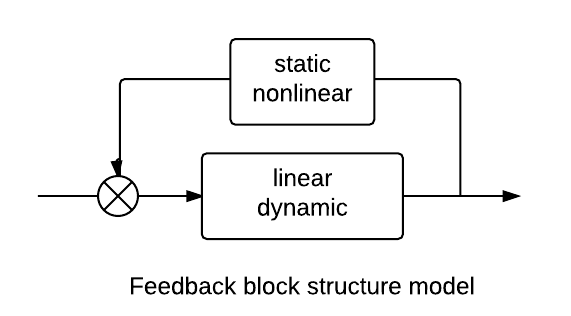
\includegraphics[height=3cm]{feedback.png}
    \caption{feedback model}
\end{center} \label{Wiener}
\end{figure}
\vspace{-.5cm}
\noindent 
However, almost all these methods rely on previous knowledge that the system under study
has a specific structure \cite{NARMAXbook}. Besides,
most researches on block-structured models focus on SISO, MISO, and MIMO systems,
instead of PDE systems.
They directly model the transformation from the system input to the
system output, failing to take advantage of the PDE form expressed by Eqn\eqref{first equation}. 
Indeed, block-structured models may overly restrict the form of the model.
We would prefer a more general description of the model.
\\

\noindent Volterra models, a.k.a. Volterra series models, use polynomials to represent 
the system. It is similar to a Taylor series but has a memory effect \cite{volterra 1, volterra 2}.
If we think of Taylor series as a functional that applies to a snapshot of $u(x,t)$ for
a fixed $t$, then the Volterra series can be thought as a functional that applies to
the whole history of $u(x,t)$ \cite{NARMAXbook}.
We call a Volterra model of $k$th order if the polynomial is of $k$th order.
For example, if $F = F(x(t))$, then an $m$th order Volterra model on
$t\in [0,T]$
would approximate $F$ as
\begin{equation}\begin{split}
    F &\approx h_0 + \sum_{k=1}^m H_k x(t)\\
    H_k x(t) &= \int_{\tau_1=0}^T \cdots \int_{\tau_k=0}^T 
    h_k(\tau_1, \cdots, \tau_k) \prod_{j=1}^k x(t-\tau_j) d\tau_j
\end{split}\end{equation}
More generally, for $F = F(x_1(t),\cdots, x_n(t))$, an $m$th order Volterra model would be
\cite{volterra 1}
\begin{equation}\begin{split}
    F & \approx h_0 + \sum_{p=1}^m H_p \mathbf{x}(t)\\
    H_p \mathbf{x}(t) &= \sum_{
        \begin{split}
           & \scriptscriptstyle k_1\ge 0,\cdots,k_n\ge 0\\[-2.3mm]
           & \scriptscriptstyle k_1+\cdots+k_n=p
        \end{split}
    }
    \int_{\tau_{j_1}} \cdots \int_{\tau_{j_n}} 
    \prod_{j_1=1}^{k_1} \cdots \prod_{j_n=1}^{k_n}
    h_{k_1,\cdots,k_n}(\tau_{j_1}, \cdots, \tau_{j_n})
    x_1(t-\tau_{j_1}) d\tau_{j_1}\, \cdots\,
    x_n(t-\tau_{j_n}) d\tau_{j_n}
\end{split}\end{equation}
A special case of Volterra model is a \emph{memoryless} polynomial expansion, written as
\begin{equation}
    H_p \mathbf{x}(t)= \sum_{
        \begin{split}
           & \scriptscriptstyle k_1\ge 0,\cdots,k_n \ge 0\\[-2.3mm]
           & \scriptscriptstyle k_1+\cdots+k_n=p
        \end{split}
    }
    h_{k_1,\cdots,k_n}
    x_1^{k_1}(t) \cdots x_n^{k_n}(t)
    \label{polynomial Volterra}
\end{equation}
As discussed in section \ref{psetup}, our unknown flux function
$F_i$ only depends on \\
$\mathcal{D}u = \left\{u_1, \nabla u_1 , \cdots, \nabla^{i_1} u_1; \cdots;
u_n, \nabla u_n,\cdots, \nabla^{i_n} u_n\right\}$, rather than depending on the time history of $u$.
Therefore Eqn\eqref{polynomial Volterra} suffices to describe the unknown flux.\\

\noindent NARMAX models (nonlinear autoregressive moving average models with exogeneous parameters),
introduced in \cite{billings 1981}, provides a more general model description.
Initially it was invented to model a \emph{discrete} SISO system with exogeneous inputs $\mathbf{u}$
and output noise $\mathbf{e}$:
\begin{equation}
    y(t) = F[y(t-1), y(t-2), \cdots, y(t-n_y), u(t-1), u(t-2),\cdots, u(t-n_u),
    e(t-1), e(t-2), \cdots, e(t-n_e)] + e(t)
\end{equation}
Hereby NARMAX' name.
While NARMAX started as the name of a model, it has now developed into a philosophy of 
nonlinear system identification.
The philosophy consists of the following steps to identify a model \cite{NARMAXbook}:
\begin{itemize}
    \item \emph{Model representation}:  Represent $F$ by a library of terms
    \item \emph{Structure detection}:   Remove unnecessary terms in the expansion
    \item \emph{Parameter estimation}:  Fit the term coefficients
    \item \emph{Model validation}:      Check if the model's error is predictable
\end{itemize}
The first step is to expand the functional form $F$ by a \emph{linear} combination
of a library of \emph{basis} terms;
for example, using Volterra series models, wavelet decomposition \cite{Wavelet SI}, 
neural networks \cite{ANN SI}, etc. The choice of the library is up to the user's
choice. 
However, a naive proceeding to fitting the coefficients of all the terms in the library
can be computationally intractable.
Often there are only a few terms in the library that are important in the model.
So the next step is to detect those terms. 
NARMAX proceeds this step by first selecting the most important term, then
the next most important terms, and so on, until a termination criterion is met. We'll investigate
the structure detection step in greater detail in section \ref{adaptive}.
After the structure detection, NARMAX estimates the coefficients of the terms, for example using
a mean square error approach, so the output of the identified model and the 
underlying system match on the sampled inputs.
Finally, the model is validated to check if the identified model
is adequate, for example, if there is anything
predictable left in the model output's error \cite{correlation model validation}. 
Unless the model is determined adequate, the term library will be enlarged and the previous 
procedures will be conducted again.
We'll discuss the model validation step in section \ref{future work}.\\

\noindent 
We will adopt the NARMAX philosophy to identify the twin model because of two considerations.
Firstly, NARMAX is generic.
It does not pose any limitation on the model representation library beforehand.
Secondly, NARMAX is parsimonious.
It attempts to find the simplest model structure before fitting the term coefficients.
In my thesis,
we will expand the functionals $F_i$'s in Eqn\eqref{first equation}
by a library of terms.  The choices of the library will be explored.
Then we will use NARMAX philosophy to fit the $F_i$'s.
Chapter \ref{gradient_surrogate} will discuss fitting the twin model without the structure 
detection step, i.e. twin model with fixed structure.
Chapter \ref{adaptive} will focus on the structure detection.\\

\subsection{Formulation of twin model with fixed structure}
\label{general formulation}
\noindent In the parameter estimation step,
we need a \emph{criterion} to determine if the twin model matches the primal model.
Given the same inputs (controls $c$, initial conditions, boundary conditions, and exogenous 
inputs $\kappa$ and $\eta$), 
suppose the space-time solution generated by the primal model is $u$.
An ideal twin model should provide a space-time solution $\tilde{u}$ such that
$J(\tilde{u},c)$ is a good estimate of $J(u,c)$.
Therefore a straightforward criterion is to minimize the difference of the objective functions
\begin{equation}
    \left| J(\tilde{u},c) - J(u,c) \right|
    \label{minimizer false}
\end{equation}
However, computing $J$ effectively compresses the space-time solution into just one number,
where lots of information contained in $u$ would be lost \cite{hanmaster}.
To take advantage of the space-time solution, we consider the minimization of
\begin{equation}
    \frac{1}{T}
    \int_{t=0}^T\int_{\mathbf{x}\in\Omega} w^2(t,\mathbf{x}, u,\tilde{u}) (\tilde{u} - 
    u)^2 \, dtd\mathbf{x}\,,
    \label{minimizer twin model}
\end{equation}
where $w^2>0$ is a weight possibly depending on $t$, $\mathbf{x}$, $u$, and $\tilde{u}$.
Eqn\eqref{minimizer twin model}$
\rightarrow 0$ provides a sufficient condition for Eqn\eqref{minimizer false} $\rightarrow 0$,
but the reverse is not true.
We will delay the discussion of $w$ to section \ref{future work}.
Right now we assume $w\equiv 1$ for simplicity.
Notice the square on $\tilde{u}-u$: it is the most popular norm and is differentiable.
The reason of using a differentiable expression will be discussed soon in this chapter.\\

\noindent The space-time solution is discretized rather than continuous. 
If the twin model and the 
primal model use the same space-time grid, then Eqn\eqref{minimizer twin model} can be
approximated by
\begin{equation}
    \frac{1}{T}
    \sum_{i=1}^{N}\sum_{k=1}^{T} \left(\tilde{u}_{ik} - u_{ik}\right)^2 \Delta t_k
    \left| \Delta \mathbf{x}_i \right|\,,
    \label{minimizer twin model discrete}
\end{equation}
where $\left| \Delta \mathbf{x}_i \right|$ indicates the size of the grid.
If the grids are different, then a mapping $P$ from $u$ to $\tilde{u}$ is required.
In this case, Eqn\eqref{minimizer twin model discrete} would translate to
\begin{equation}
    \frac{1}{T}
    \sum_{i=1}^{N}\sum_{k=1}^{T} \left(\tilde{u}_{ik} - P(u)_{ik}\right)^2 \Delta t_k
    \left| \Delta \mathbf{x}_i \right|\,,
    \label{minimizer twin model discrete mapping}
\end{equation}
Right now, we assume the grids are the same for simplicity. In addition, we
assume the right hand side $q_s$ in the twin model is known. Extension to
unknown $q_s$ will be discussed later.\\

\noindent To sum up, the problem of constructing a twin model (with fixed structure)
is converted to the following problem:\\
\fbox{\parbox{\textwidth}{
Solve
\begin{equation}
    \xi^* = \arg\min_{\xi} L(\tilde{u}(\xi)) =
    \arg\min_{\xi} \left\{
    \frac{1}{T}
    \sum_{i=1}^{N}\sum_{k=1}^{T} \left(\tilde{u}_{ik} - u_{ik}\right)^2 \Delta t_k
    \left| \Delta \mathbf{x}_i \right|
    + \lambda \|\xi\|^2  \right\}
    \,,
    \label{objective twin model}
\end{equation}
where $u$ is the discretized space-time solution of the primal model, and $\tilde{u}$
is the discretized space-time solution of
\begin{equation}
    \frac{\partial\eta_s \tilde{u}_s(t,x)}{\partial t} + \nabla \cdot \left\{
    \sum_{k=1}^{m_s}\xi_{sk} g_{sk}(\mathcal{D} \tilde{u}, \kappa)  \right\}
    = q_s(\tilde{u},c(t,x))\,, \qquad s=1,\cdots, n\,,
    \label{first equation 2}
\end{equation}
$g_{sk}$, $k=1\cdots m_s$ are the library of basis functions for $F_s$. 
$\xi$'s are the coefficients for the basis functions. $\lambda\|\xi\|^2$
is the regularization with $\lambda>0$. $\|\cdot\|$ is the $L_2$ vector norm.
The grids of the primal model solver and the twin model solver are assumed the same.
Also, the primal model and the twin model use the same control, initial condition, 
boundary condition, and exogeneous parameters $\eta$ and $\kappa$.
}}
\\

\noindent Although the twin model method was developed for fitting a time-dependent PDE, 
the idea can be extended to time-independent PDE as well. 
Twin models for time-independent PDEs can be viewed as a special case for time-dependent
PDEs. Consider solving a time-independent PDE with an iterative solution method
with pseudo time marching (assume stability is satisfied), then
we are only interested in matching the solutions \emph{at the very last pseudo
timestep}. The formulation is given below\\

\fbox{\parbox{\textwidth}{
Solve
\begin{equation}
    \xi^* = \arg\min_{\xi} L(\tilde{u}(\xi)) =
    \arg\min_{\xi} \left\{
    \sum_{i=1}^{N}\left(\tilde{u}_{ik} - u_{ik}\right)^2
    \left| \Delta \mathbf{x}_i \right|
    + \lambda \|\xi\|^2 \right\}
    \,,
    \label{objective twin model steady}
\end{equation}
where $u$ is the discretized spatial solution of the primal model, and $\tilde{u}$
is the discretized spatial solution of
\begin{equation}
    \nabla \cdot \left\{
    \sum_{k=1}^{m_s}\xi_{sk} g_{sk}(\mathcal{D} \tilde{u}, \kappa)  \right\}
    = q_s(\tilde{u},c(x))\,, \qquad s=1,\cdots, n\,,
    \label{first equation 2 steady}
\end{equation}
$g_{sk}$, $k=1\cdots m_s$ are the library of basis functions for $F_s$. 
$\xi$'s are the coefficients for the basis functions. 
$\lambda\|\xi\|^2$ is the regularization with $\lambda>0$.
$\|\cdot\|$ is the $L_2$ vector norm.
The grids of the primal model solver and the twin model solver are assumed the same.
Also, the primal model and the twin model use the same control, 
boundary condition, and exogeneous parameters $\kappa$.
}}
\\

\subsection{Adjoint-based parameter estimation of twin model}
\noindent Similar to optimizing $J$, constructing a twin model is another optimization problem. 
However, the latter problem is easier to solve because the twin model, Eqn\eqref{first equation 2},
is an open-box model. As mentioned in chapter \ref{intro}, open-box models admit efficient
gradient-driven optimization, where the gradient $\frac{dL}{d\xi}$
can be computed by adjoint method \cite{adjoint, cont discretize adjoint}.
To obtain the gradient, we first linearize $L$ in Eqn\eqref{objective twin model},
\begin{equation}
    \delta L = \left(\frac{d L}{d \tilde{u}}\right)^T \delta \tilde{u}
\end{equation}
Then we linearize the residual $\tilde{R}(\tilde{u},\xi)$ of Eqn\eqref{first equation 2},
\begin{equation}
    \frac{\partial \tilde{R}}{\partial \tilde{u}} \delta \tilde{u}
    + \frac{\partial \tilde{R}}{\partial \xi} \delta \xi = 0
\end{equation}
Introduce a Lagrange multiplier $\lambda$, a.k.a. \emph{adjoint state}, we have
\begin{equation}\begin{split}
    \delta L &= \left(\frac{d L}{d \tilde{u}}\right)^T \delta \tilde{u}
    - \lambda^T \left(\frac{\partial \tilde{R}}{\partial \tilde{u}} \delta \tilde{u}
    + \frac{\partial \tilde{R}}{\partial \xi}\delta \xi\right)\\
    &= -\left( \lambda^T \frac{\partial \tilde{R}}{\partial \xi}\right) \delta \xi
    + \left( \left(\frac{d L}{d \tilde{u}}\right)^T 
        - \lambda^T \frac{\partial \tilde{R}}{\partial \tilde{u}}
    \right)\delta \tilde{u}
\end{split}\end{equation}
Therefore, the adjoint state satisfies the \emph{adjoint equation}
\begin{equation}
    \left(\frac{\partial \tilde{R}}{\partial \tilde{u}}\right)^T \lambda = \frac{d L}{d\tilde{u}}\,,
\end{equation}
and the gradient is given by
\begin{equation}
    \frac{dL}{d \xi} = -
    \left(\frac{\partial \tilde{R}}{\partial \xi}\right)^T \lambda
\end{equation}

\subsection{Basis library for twin model}
\label{basis selection}
\noindent Next, we consider choosing an appropriate basis library $g$.
As mentioned in section \ref{SI review}, the basis functions can be chosen
as a Volterra series. In this section we provide a different basis library
from the viewpoint of multiresolution analysis.
For simplicity, we start from a one dimensional function $F(\tilde{u})$, 
$\tilde{u}\in \mathbb{R}$.
Theoretically, many fuction approximation methods can be chosen for $g$, such as polynomial 
approximation, Fourier series approximation, and wavelet approximation. 
We will focus on the wavelet approximation. In the following we will apply the theory 
of wavelet approximation to our problem, then we will discuss the reasons for choosing 
wavelet approximation.\\

\noindent Wavelet approximation can be explained by Mallat's \emph{multiresolution analysis (MRA)}
\cite{wavelet mallat}. In one dimension,
MRA is an increasing sequence of closed function spaces $\{V_j\}_{j\in \mathbb{Z}}$
which approximates $L^2(\mathbb{R})$.
$V_{j}$ approximates functions with increasing resolutions as $j$ increases.
The spaces satisfy the following properties:
\begin{equation*}\begin{split}
    &\textrm{MRA}\, 1\qquad \cdots \subset V_{-1} \subset V_0 \subset V_1 \subset \cdots\\
    &\textrm{MRA}\, 2\qquad 
                    \bigcup_{j\in \mathbb{Z}} V_j \;\; \textrm{is dense in }\; L^2(\mathbb{R})\\
    &\textrm{MRA}\, 3\qquad f(x) \in V_j \Leftrightarrow f(2x) \in V_{j+1}, \; j\in \mathbb{Z}\\
    &\textrm{MRA}\, 4\qquad f(x) \in V_j \Leftrightarrow f(x-\frac{k}{2^j}) \in V_{j},
                    \; j\in \mathbb{Z},\, k\in \mathbb{Z}
\end{split}\end{equation*}
In wavelet theory, the orthonormal basis for $V_j$ is given by
\begin{equation}
    \phi_{j,k}(x) = 2^{j/2} \phi(2^j x-k) \,,\quad k \in \mathbb{Z}
\end{equation}
$\phi_{0,0}$ is called the \emph{scaling function}. 
Projecting a function $f\in L^2(\mathbb{R})$ on the $V_j$ gives
\begin{equation}\begin{split}
    P_{V_j} f &= \sum_{k\in\mathbb{Z}} \left<f, \phi_{j,k}\right> \phi_{j,k}\\
    & = \sum_{k\in\mathbb{Z}} \left( \int_{\mathbb{R}} f(x) \phi_{j,k}(x) \,\textrm{d}x \right)\;
    \phi_{j,k}
    \label{scaling projection}
\end{split}\end{equation}
\noindent Scaling functions can be either discontinuous (e.g. Haar wavelet \cite{haar}) 
or continuous (e.g. Meyer wavelet \cite{Analytic Meyer}). 
Because we desire differentiability of the twin model, we will focus on
continuous scaling functions.
As an example, we show the Meyer wavelet scaling function and its spectrum.
\begin{figure}[H]\begin{center}
    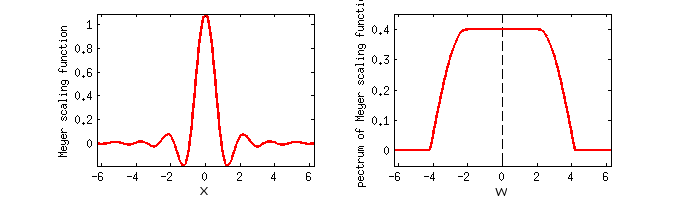
\includegraphics[height=4cm]{meyer.png}
    \caption{Meyer wavelet scaling function and its spectrum}
\end{center}\label{fig:Meyer}\end{figure}
\noindent 
$\phi_{j,k}(x)$ is localized in the frequency domain, and can be seen as a low pass filter.
Projecting a function $f \in L^2(\mathbb{R})$
onto $V_j$ gives a bandlimited approximation of $f$.
As $j$ increments by $1$, the bandwidth of the low pass filter will increase by a
factor of $2$,
so does the approximation resolution.
Besides, $\phi_{j,k}(x)$ is localized in $x$, i.e.
$\phi_{j,k}(x)\rightarrow 0$ as $x\rightarrow \pm \infty$.
Given $j$ and $k$,
$\left<f,\phi_{j,k}\right>$ effectively controls 
the shape of $P_{V_j} f$ only within a bounded domain centered at $\frac{k}{2^j}$.
This will be an important property when we discuss the concept of \emph{excited parameter domain}
in section \ref{adaptive}. In practice, it's infeasible and unnecessary to include all $\phi_{j,k}$
$k\in\mathbb{Z}$ into the basis library for a given $j$.
For example, in the 1D water-oil displacement process 
\cite{Buckley Leverett}, the water saturation $u$ satisfies $0\le u\le 1$. Therefore, it's 
unnecessary to consider $k$ for which $\frac{k}{2^j} \gg 1$ or $\frac{k}{2^j} \ll 0$.
We will discuss this topic in greater detail in section \ref{adaptive}.\\

\noindent In Eqn\eqref{first equation} and Eqn\eqref{first equation 2}, we notice that
adding a constant to $F$'s and $g$'s does not change the equations. In other words,
it suffices to approximate the flux functions' gradients instead of the flux function value.
Therefore, we consider the following functions:
\begin{equation}
    \bar{\phi}_{jk}(x) = \int_{-\infty}^x \phi_{j,k}(\tau)\;\textrm{d}\tau
\end{equation}
The gradient of $\bar{\phi}_{jk}(x)$ is local in frequency and
local in $x$. 
In this section, we will use $\left\{\bar{\phi}_{jk}\right\}$, $k\in \mathbb{Z}$ with
a fixed $j$ as the basis library for the flux function. \\

\noindent For flux functions $F(\tilde{u})$, $\tilde{u}\in \mathbb{R}^n$, $n>1$, the analogy of
basis functions is straightforward.
The MRA for $L^2(\mathbb{R}^n)$ is 
$V_{j_1}\otimes V_{j_2}\otimes \cdots \otimes V_{j_n}$, with
$\{j_1,j_2,\cdots,j_n\}\in \mathbb{Z}^n$ \cite{wavelet mallat, Dijkema book}.
Given $\mathbf{j} = \left\{j_1,\cdots,j_n\right\}$, The basis is
\begin{equation}
   \mathbf{\phi}_{\mathbf{j},\mathbf{k}} = \phi_{j_1,k_1}(x_1)\cdots \phi_{j_n,k_n}(x_n)\,,
   \quad \mathbf{k}\in\mathbb{Z}^n
\end{equation}
Therefore, the basis for the twin model flux function is
\begin{equation}
   \bar{\mathbf{\phi}}_{\mathbf{j},\mathbf{k}} = \bar{\phi}_{j_1,k_1}(x_1)
   \cdots \bar{\phi}_{j_n,k_n}(x_n)\,,
   \quad \mathbf{k}\in\mathbb{Z}^n
   \label{basis flux wavelet}
\end{equation}
Below we plot $\bar{\phi}_{0,0}(x)$ and $\bar{\phi}_{\mathbf{0},\mathbf{0}}(x_1,x_2)$ 
integrated from Meyer scaling function.
\begin{figure}[H]\begin{center}
    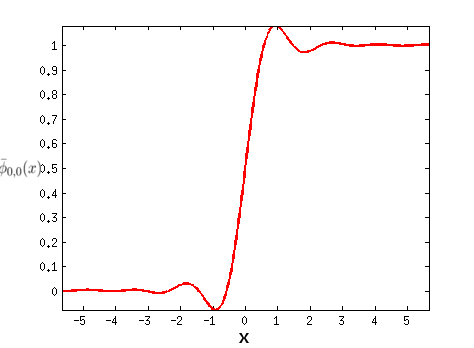
\includegraphics[height=5cm]{basis.png}
    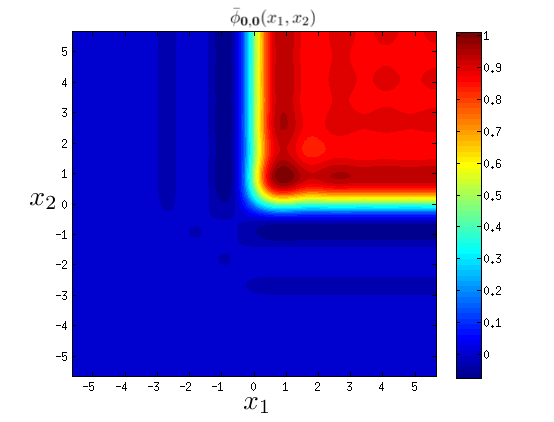
\includegraphics[height=5cm]{basis_2D.png}
\end{center}
\caption{$\bar{\phi}_{0,0}$ in 1D and 2D, integrated from Meyer wavelet scaling function}
\label{fig:Meyer Basis}
\end{figure}
\noindent Clearly, using Eqn\eqref{basis flux wavelet} as the basis for the flux functions
will be problematic for high dimensional $\mathbf{x}$. We will address this problem
in section \ref{adaptive}.\\

\noindent Although function approximation with wavelet scaling function has mathematical
rigor, $\bar{\phi}$'s are not ideal bases for our problem. Firstly, the
integral of 1D scaling function is rippled, as can be seen in the Meyer wavelet example.
This is due to the \emph{localization in frequency}
property of scaling functions, known as the Gibbs phenomenon. 
The rippled flux may cause shock waves in hyperbolic equation simulations.
Indeed, the property of localization in frequency is not necessary in our
twin model problem.
Secondly, generally $\bar{\phi}$ does not have an analytical expression. 
So $\bar{\phi}$ must be evaluated by numerical integration or interpolation
using a lookup table, which can be more computationally intensive than
anlytical expressions. Therefore, we prefer a \emph{monotonic} and \emph{analytical}
 approximation for $\bar{\phi}$.\\

\noindent We choose a sigmoid function to replace $\bar{\phi}_{0,0}$:
\begin{equation}
    \bar{\phi}_{0,0}(x) = \frac{1}{2}\left(\tanh(\beta x)+1\right)\,,
\end{equation}
where $\beta$ is a constant determining the gradient of the function at $x=0$.
And
\begin{equation}
    \bar{\phi}_{j,k}(x) = \frac{1}{2} \left\{
        \tanh\left(\beta(2^j x-k)\right) +1
    \right\}
    \label{phijk}
\end{equation}
Or if we don't specify resolution on a dyadic grid $2^j$, we can write Eqn\eqref{phijk} as
\begin{equation}
    \bar{\phi}_{r,k}(x) = \frac{1}{2} \left\{
        \tanh\left(\beta(r x-k)\right) +1
    \right\}\,,
    \label{phirk}
\end{equation}
where $r>0$.
Without further specifications we'll choose $\beta=1.5$.
Below we plot $\bar{\phi}_{0,0}(x)$ and $\bar{\phi}_{\mathbf{0},\mathbf{0}}(x_1,x_2)$ 
using the sigmoid function.
\begin{figure}[H]\begin{center}
    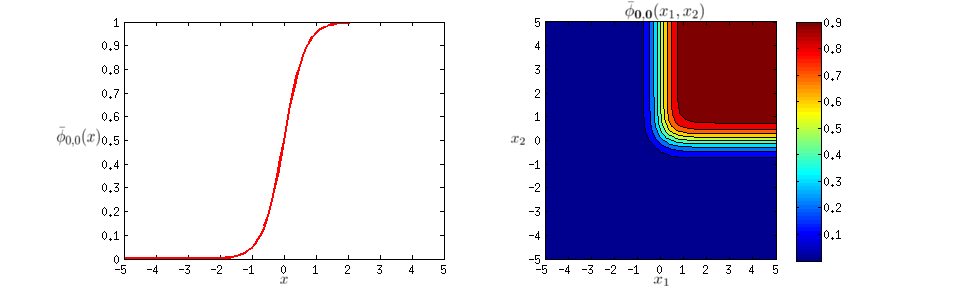
\includegraphics[height=5cm]{sigmoid_basis.png}
    \caption{$\tanh$ sigmoid function in 1D and 2D}
    \label{fig:sigmoid basis}
\end{center}\end{figure}


\subsection{Numerical example: twin model with fixed structure}
\label{fixed numerical example}
In this section we demonstrate a numerical example for fitting a twin model with fixed structure.
Consider a 1D Buckley-Leverett equation
\begin{equation}
    \frac{\partial u}{\partial t} + \frac{\partial F(u)}{\partial x} = 0\,\quad x\in[0,1]\,,\; t\in[0,1]
    \label{BL eqn}
\end{equation}
with periodic boundary condition
\begin{equation}
    u(x=0) = u(x=1)
\end{equation}
and initial condition
\begin{equation}
    u(t=0) = u_0
\end{equation}
Buckley-Leverett equation is a simple model for 1D, two-phase, porous media flow driven by
capillary pressure and Darcy's law \cite{Buckley Leverett}. $u$
indicates one phase's saturation and $0\le u\le 1$.
The flux function $F(u)$ depends on the phases and the porous media. 
A popular $F(u)$ is
\begin{equation}
    F(u) = \frac{u^2}{1+A(1-u)^2}\,,
    \label{BL flux}
\end{equation}
where $A$ is a constant. In the following we assume the blackbox simulation
solves Eqn\eqref{BL eqn} with the flux given by Eqn\eqref{BL flux}, and $A=2$.
\\

\noindent Assume $F(u)$ is unknown, we will fit a twin model 
using the blackbox simulation.
As discussed in section \ref{general formulation} and
\ref{basis selection}, the twin model can be written as
\begin{equation}
    \frac{\partial \tilde{u}}{\partial t} + \frac{\partial}{\partial x}\,
    \left(\sum_{k=1}^m \xi_k \bar{\phi}_{r,k}(\tilde{u})\right) = 0
\end{equation}
with the same initial and boundary conditions. We will
use Eqn\eqref{phirk} for $\bar{\phi}$. Both the black-box simulation
and the twin model use a second order finite volume discretization and 
Crank-Nicolson time integration scheme.\\

\noindent We need to determine $r$ and the range for $k$ a prior. 
A larger $r$  means higher resolution of the flux, but the twin model will be
more computationally costly to fit. For this example,
we specify $r=10$. Besides, not all $k\in \mathbb{Z}$
are required in the twin model. As mentioned before, the gradient of
each basis indexed by $k$ is non-zero only around $[\frac{k}{r}-\frac{1}{\beta r},
\frac{k}{r}+\frac{1}{\beta r}]$. In our problem, $0\le u\le 1$, so it suffices
to choose corresponding $k$'s. We will choose $k=-1,0,\cdots, 11$.\\

\noindent The objective of fitting the twin model is given in Eqn\eqref{objective twin model},
and is itself an optimization.
We use an automatic differentiation module \textit{numpad} \cite{numpad} to compute
$\frac{dJ}{d\xi_k}\,, k=1,\cdots, m$.
Since the gradient information is available, we consider using a quasi-Newton method
for the optimization. Quasi-Newton methods build the Hessian approximation iteratively 
using gradient, and can greatly accelerate convergence \cite{Quasi-Newton Review}.
When the degree of freedom of the optimization is high, the memory required to 
store the Hessian matrix can be large. To reduce the memory requirement, 
we can use the \emph{low-memory Broyden-Fletcher-Goldfarb-Shannon} (L-BFGS) algorithm
\cite{nlopt, LBFGS, Eric master thesis}. 
L-BFGS approximates the Hessian using only the gradients at newer previous iterations,
and inverse the approximated Hessian efficiently using the Sherman-Morrison formula.
For this work, we
use the implementation of L-BFGS in Nlopt \cite{nlopt}.\\

\noindent Although the objective is to minimize 
$
\sum_{i=1}^{N}\sum_{k=1}^{T} \left(\tilde{u}_{ik} - u_{ik}\right)^2 \Delta t_k
\left| \Delta \mathbf{x}_i \right|
$, we will not use it as the objective function directly and perform optimization
in one shot. If $\tilde{F}(u)$ deviates from $F(u)$ a lot, then $\tilde{u}(x,t)$
can deviate from ${u}(x,t)$ significantly even at a small $t$. 
Therefore, solving the twin model and its adjoint in $t=[0,T]$ without
an educated $\tilde{F}(u)$ can be a waste of computation 
resources. To improve efficiency, we propose a progressive optimization
procedure:\\
\fbox{\parbox{\textwidth}{
\begin{algorithm}[H]
    $\xi^*=\mathbf{0}$\;
    Set integers $2= i_1< \cdots < i_M=T$\;
    \For{$I=i_1,\cdots, i_M$}{
        Optimize
        $$
           \xi^* \leftarrow \arg\min_{\xi} 
           \sum_{i=1}^{N}\sum_{k=1}^{I} \left(\tilde{u}_{ik} - u_{ik}\right)^2 \Delta t_k 
           \left| \Delta \mathbf{x}_i \right|
        $$
        with initial guess $\xi^*$.
  }
  \caption{Progressive optimization procedure}
  \label{progressive algo}
\end{algorithm}
}}\\

\noindent Notice $k=1$ corresponds to the initial condition. Since the twin model
uses the same initial condition as the black-box model, $\tilde{u}_{i1} - u_{i1}$
is always zero.
Choosing the integer sequence $i_1,\cdots,i_M$ can be problem dependent.
Our experience shows the sequence should be denser at small $i$, and sparser at larger $i$.
The tolerance of each sub-optimization problem does not need to be tight,
except for the last iteration where $I=T$.
In our problem, we use $i_l = \min\left\{ 1+2^l, T\right\}$,
a relative tolerance of $10\%$, and maximum $10$ iterations for the sub-optimization problems.\\

\noindent The initial condition is shown in Fig \ref{fig:initial condition}. Notice
$u_0$ does not cover the entire range of 
$0\le u\le 1$: we have $\max(u_0) =0.89$, $\min(u_0) = 0.07$.
\begin{figure}[H]\begin{center}
    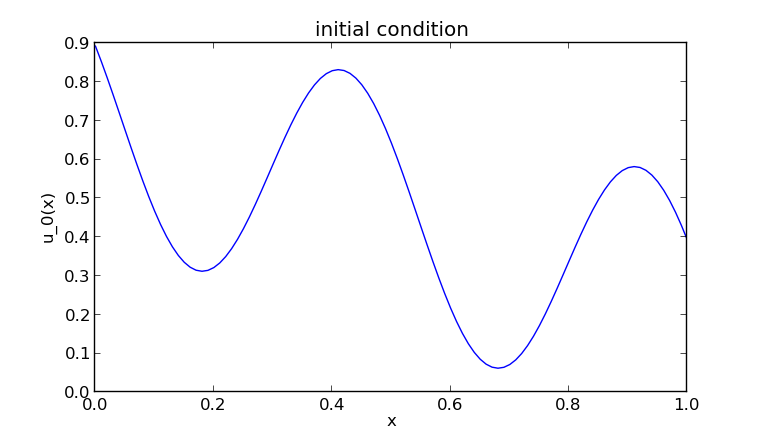
\includegraphics[height=4cm]{initial_condition.png}
    \caption{Initial condition $u_0(x)$}
    \label{fig:initial condition}
\end{center}\end{figure}
\noindent In Fig \ref{fig:flux compare} we compare the converged twin model's flux $\tilde{F}(u)$ and its gradient $\frac{d\tilde{F}}{du}$
with $F(u)$ and $\frac{dF}{du}$. The range
$u\in [\min(u(t,x)), \max(u(t,x))]$ is colored green.
\begin{figure}[H]\begin{center}
    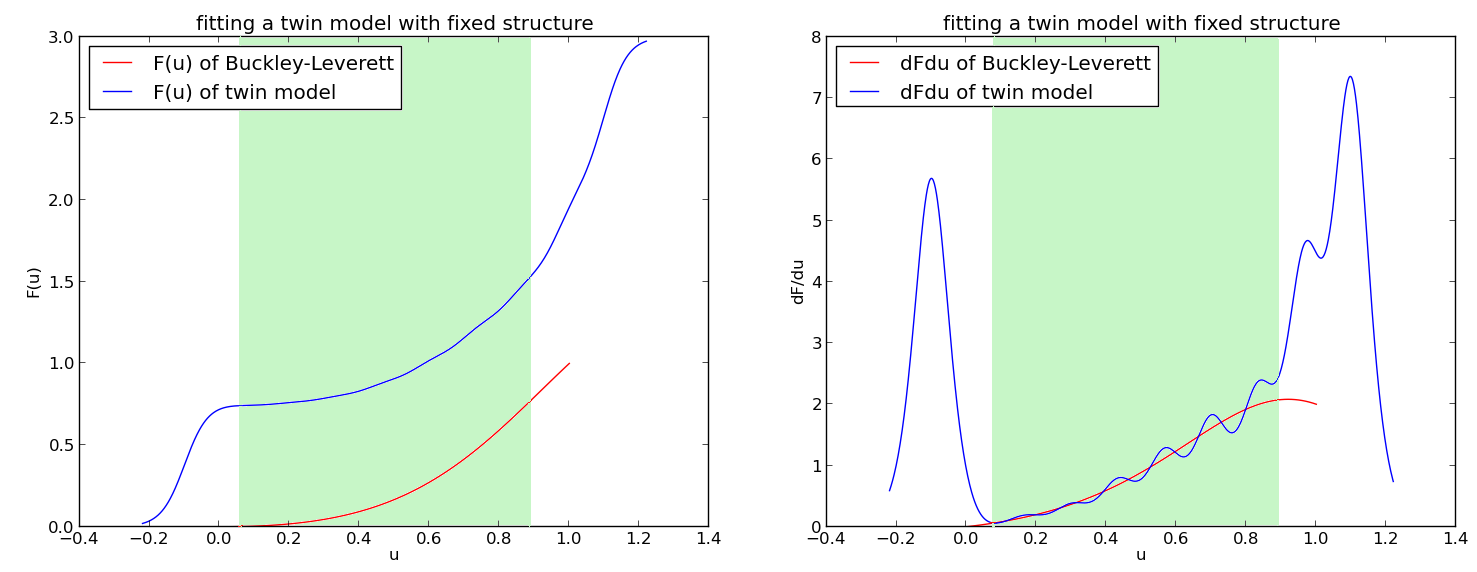
\includegraphics[height=5cm]{fit_flux_2.png}
    \caption{Compare $F(u)$ and $\frac{dF}{du}$ with $\tilde{F}(u)$ and $\frac{d\tilde{F}}{du}$}
    \label{fig:flux compare}
\end{center}\end{figure}
\noindent In Fig \ref{fig:sol compare} we compare the solution $u(t,x)$ with the converged
twin model's solution $\tilde{u}(t,x)$.
\begin{figure}[H]\begin{center}
    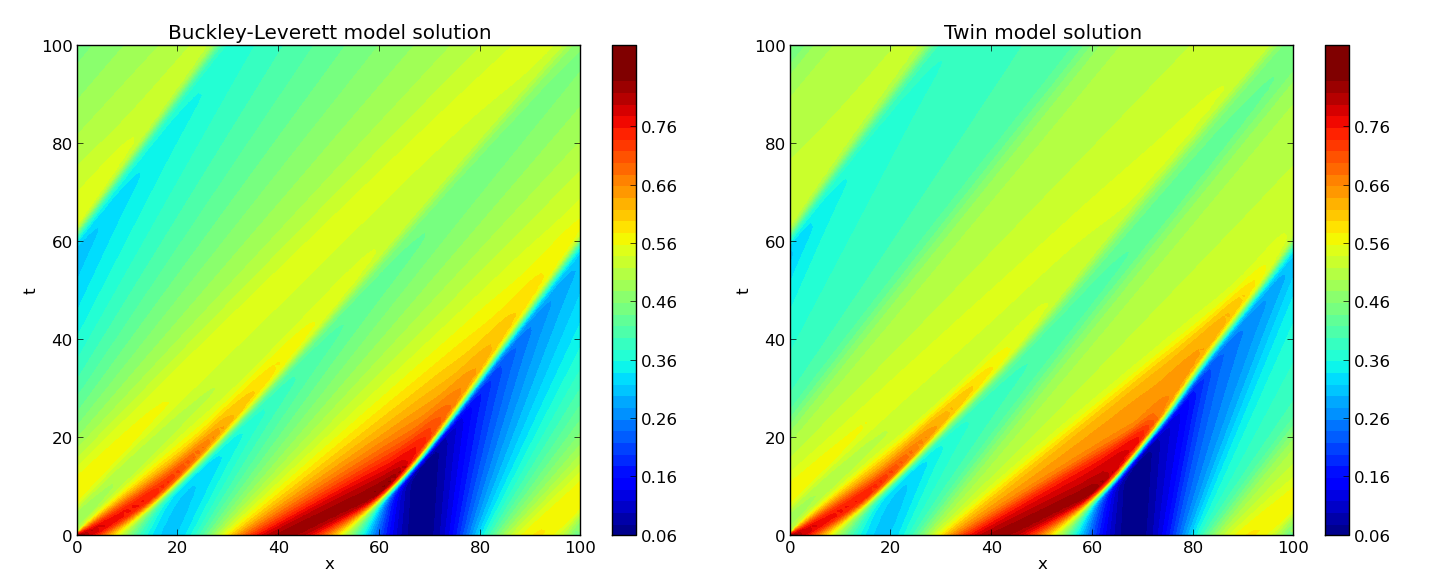
\includegraphics[height=5cm]{BL_sol.png}
    \caption{Compare $u(t,x)$ with $\tilde{u}(t,x)$}
    \label{fig:sol compare}
\end{center}\end{figure}

\noindent If we increase the flux resolution, the flux and the solution should have a better fit.
For example, we use $r=30$, $k=-3,\cdots,33$. The flux comparison is shown in Fig
\ref{fig:flux compare 30}
\begin{figure}[H]\begin{center}
    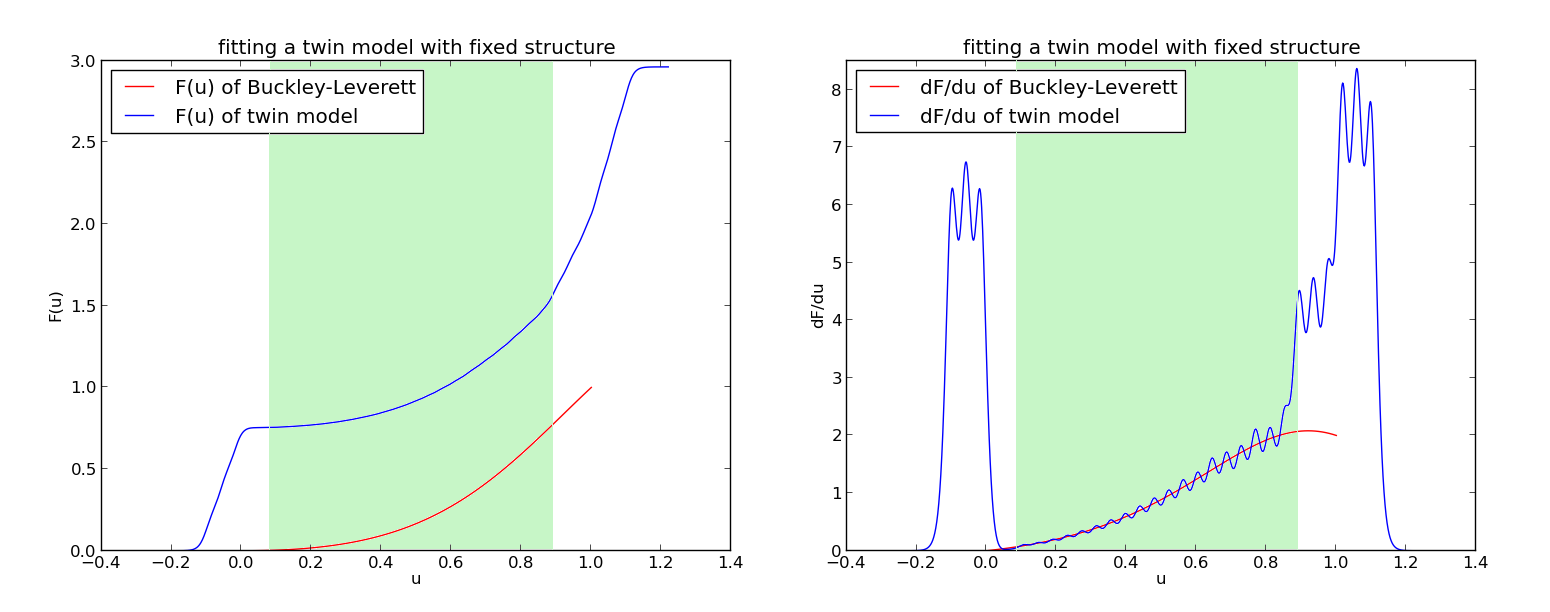
\includegraphics[height=5cm]{fit_flux_30_1.png}
    \caption{Compare $F(u)$ and $\frac{dF}{du}$ with $\tilde{F}(u)$ and $\frac{d\tilde{F}}{du}$
             with higher flux resolution}
    \label{fig:flux compare 30}
\end{center}\end{figure}
\noindent The solution comparison is shown in Fig \ref{fig:sol compare 30}
\begin{figure}[H]\begin{center}
    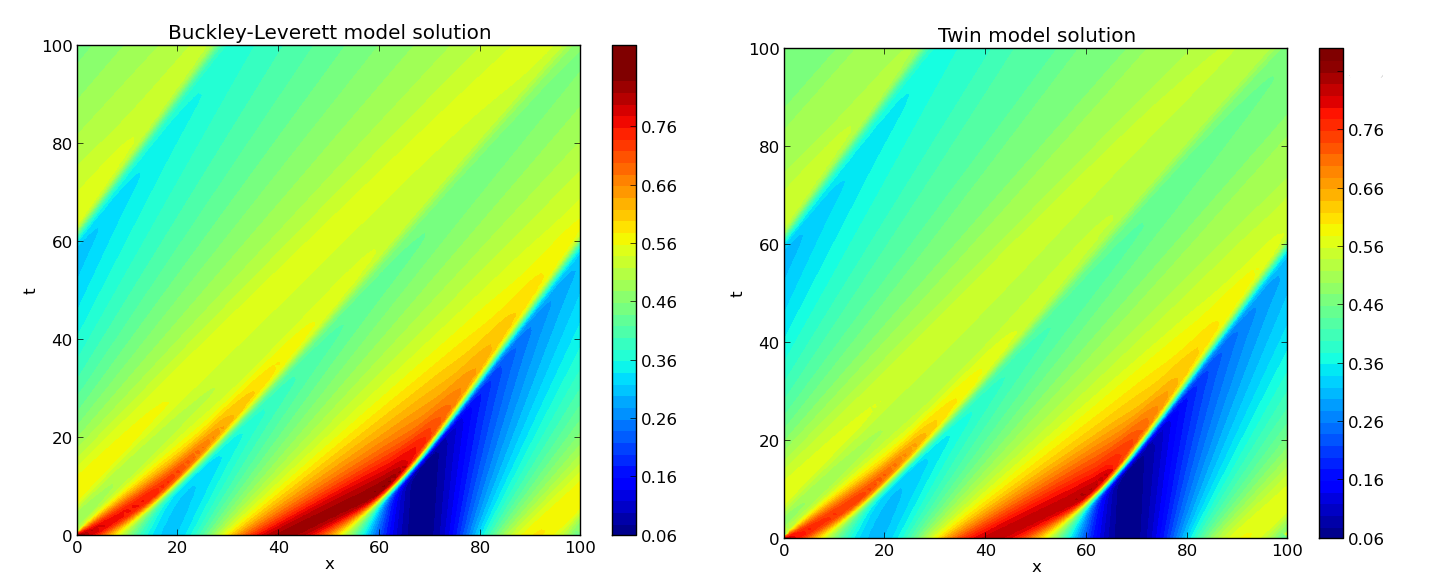
\includegraphics[height=5cm]{BL_sol_30.png}
    \caption{Compare $u(t,x)$ with $\tilde{u}(t,x)$ with higher flux resolution}
    \label{fig:sol compare 30}
\end{center}\end{figure}
\noindent Comparing Fig \ref{fig:flux compare}, \ref{fig:sol compare} 
with Fig \ref{fig:flux compare 30}, \ref{fig:sol compare 30}, we observe a refined flux basis 
gives a more accurate twin model.
However, we seek for an educated way to adaptively refine the
basis and to control the computation cost.
Therefore we will investigate \emph{twin model with adaptive structure}
in the next section.

\subsection{Twin model with adaptive structure}
\label{adaptive}
A twin model with adaptive structure should be able to adaptively
refine its basis $\bar{\phi}$ on-the-fly during fitting the basis coefficients $\xi$.
For example, in section \ref{fixed numerical example}'s numerical example,
the value of $u(t,x)$, $t\in[0,T],\,x\in[0,1]$ is bounded, i.e.
$0< u_{\min}\le u(t,x)\le u_{\max} < 1$; therefore as long as 
$\nabla\tilde{F}(u) = \nabla F(u)$ for $u\in[u_{min},u_{max}]$, we will have
$\tilde{u}(t,x) = u(t,x)$ for $t\in[0,T]$ and $x\in[0,1]$.
In other words, in the numerical example, $\nabla \tilde{F}(u) = \nabla F(u)$ for $u\in [0,1]$
is a sufficient but not necessary condition
for $\tilde{u}(t,x) = u(t,x)$. 
Intuitively, for some domains $u$, $\nabla \tilde{F}(u)$ has to approximate $\nabla F(u)$
accurately in order to give a good space-time solution match.
We will call such domains \emph{excited domain}, written as $\mathcal{E}$. 
Notice the excited domain is not a domain of space or time.  
Clearly $\mathcal{E}$ depends on $u(t,x)$.
For $u$ not inside $\mathcal{E}$,
$\nabla \tilde{F}(u)$ will have little or no effect on the solution match; therefore
we may not certify $\nabla \tilde{F}(u)$'s accuracy outside $\mathcal{E}$
no matter how closely the solutions match.
As mentioned in section \ref{basis selection}, we are interested in the problem of basis
selection. Basis selections should only be navigated to $\mathcal{E}$.\\

\noindent To start with, 
consider a primal model solving the Eqn\eqref{first equation}, and a twin model solving
\begin{equation}
    \frac{\partial\tilde{u}(t,x)}{\partial t} + \nabla \cdot 
    \tilde{F}(\mathcal{D} \tilde{u}, \kappa) 
    = q(\tilde{u},c(t,x))\,, \qquad i=1,\cdots, n\,,
    \label{twin equation def}
\end{equation}
with the same initial condition, boundary condition, and controls. We define $\mathcal{E}$ by
its complement $\bar{\mathcal{E}}$:\\
\fbox{\parbox{\textwidth}{
\begin{definition}
    Given a primal model, its discretized solution $u(t,x)$, and
    a twin model Eqn\eqref{twin equation def}.
    The excited domain $\mathcal{E}$ is a domain of $\tilde{F}(\cdot)$.
    Let the complement of $\mathcal{E}$ be $\bar{\mathcal{E}}$.
    Consider a perturbed twin model flux $\tilde{F}_{\epsilon\delta}(\cdot) =F(\cdot)+ \epsilon
    \delta(\cdot)$, $\epsilon\in \mathbb{R}, \delta\in L_2(\mathbb{R}^n)$.
    The perturbed twin model gives the discretized solution $\tilde{u}_{\epsilon\delta}$.\\

    A set $e \subseteq \bar{\mathcal{E}}$ if and only if
    $$ \frac{1}{T}
    \sum_{i=1}^{N}\sum_{k=1}^{T} \left(\tilde{u}_{\epsilon\delta, ik} - u_{ik}\right)^2 \Delta t_k
    \left| \Delta \mathbf{x}_i \right|$$
    is independent of $\epsilon$ for
    any $\delta$ with $\textrm{support}[ \delta] = e$.
\end{definition}
}}\\

\noindent This definition requires $F$ a prior, therefore it is not directly implementable.
In practice, we have to replace $\tilde{F}$'s baseline $F$ with some approximation.
The definition also requires enumeration of all possible $\delta$ to validate $\mathcal{E}$.
In practice, we have to choose a finite set of $\delta$, for example using the basis function library
$\bar{\phi}$.
However, even with a finite set of $\delta$, we should not validate $\mathcal{E}$ 
with this definition numerically.
As mentioned in section \ref{fixed numerical example}, unless $\tilde{u}(\tau)$
is reasonably close to $u(\tau)$, it does not make sense to keep solving the twin model for $t>\tau$.
Therefore, we should not let $\tilde{u}$ deviates from $u$ a lot.
\\

\noindent To restrict $\tilde{u}$ from large deviation to $u$, we propose a \emph{global-local
error} approach for basis selection.
Define \emph{global error}:
\begin{equation}
    Err_{G} = 
    \frac{1}{T}\sum_{i=1}^{N}\sum_{k=1}^{T} \left(\tilde{u}_{ik} - u_{ik}\right)^2 \Delta t_k
    \left| \Delta \mathbf{x}_i \right|
    \label{global error}
\end{equation}
and \emph{local error}:
\begin{equation}
    Err_{L} = 
    \frac{1}{T}\sum_{i=1}^{N}\sum_{k=1}^{T} \left(\tilde{u}^\prime_{ik} - u_{ik}\right)^2 \Delta t_k
    \left| \Delta \mathbf{x}_i \right|
    \label{local error}
\end{equation}
Here $u$ is the \emph{one-shot} solution of the 
twin model solving from $t=0$ to $t=T$ with initial condition $u_0$.
$\tilde{u}^\prime_k$ is the solution of the twin model at $t=t_{k}$, solving from $t=t_{k-1}$
with initial condition $u_{k-1}$, for just one timestep. In other words, 
we solve $\tilde{u}^\prime$ with restart for every timestep, whose
initial condition is given by $u$ at a previous timestep.
We illustrate the idea in Fig \ref{fig:tmodelrestart}.
\begin{figure}[H]\begin{center}
    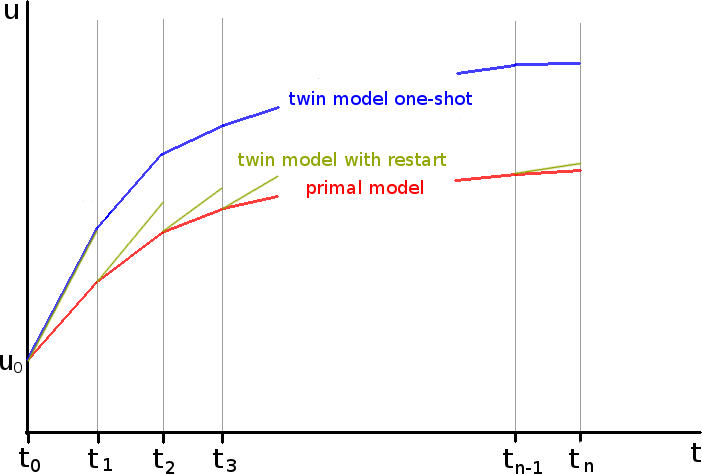
\includegraphics[height=5cm]{sketch2.png}
    \caption{illustration of twin model with restart.}
    \label{fig:tmodelrestart}
\end{center}
\end{figure}

\noindent If we are able to bound $Err_G$ with $Err_L$, we are guaranteed a good solution
match even if we do not solve for the one-shot solution $\tilde{u}$. Under what condition
can we bound $Err_G$? We give the following theorem.\\
\fbox{\parbox{\textwidth}{
\begin{theorem}
    Consider the timestepwise mapping of the twin model
    \begin{equation}
        G:\, \mathbb{R}^n\mapsto\mathbb{R}^n,\, \tilde{u}^i\rightarrow 
        G\tilde{u}^i = \tilde{u}^{i+1}\,,\quad i=1,\cdots, n\,.
    \end{equation}
    If $G$ is a Lipschitz continuous mapping with constant $\alpha$
    \begin{equation}
        \|Gx-Gy\|_{L_2} \le \alpha \|x-y\|_{L_2}
    \end{equation}
    then 
    \begin{equation}
        Err_G \le (1+\alpha+\cdots+\alpha^{n-1}) Err_L\,.
    \end{equation}
    If $\alpha < 1$, then
    \begin{equation}
        Err_G < \frac{1}{1-\alpha}Err_L
    \end{equation}
    \label{theorem: 1}
\end{theorem}
}}\\

\noindent In practice, the assumption of $\alpha<1$ may not be
guaranteed. Therefore a small local error may not guarantee a small global error,
for example for chaotic dynamical systems.
Therefore, we only consider the local error as a tool to select basis, not a tool
to finalize the twin model. After selecting
the basis using the local error metric, 
we will still use the global error metric to fit the twin model, for example
using algorithm \ref{progressive algo}.\\

\noindent Using the local error metric, we are able to reduce the twin model
into solving a series of one-timestep problems with restart. But in each one-timestep
problem, the numerical implementation of $\nabla\cdot$ in Eqn\eqref{twin equation def}
is nonlinear. If we approximate $\nabla\cdot$ linearly, we will be able to 
use the wealth of knowledge of linear system basis selection. 
Let $\nabla\cdot$ be approximated by a
finite difference operator $D$. Besides,
a stable time integration scheme of twin model's solver is necessary 
for theorem \ref{theorem: 1} to hold. Here
we let $\frac{\partial}{\partial t}$ be approximated by Backward Euler. 
Then Eqn\eqref{twin equation def} becomes
\begin{equation}
    -\frac{1}{\Delta t_k}\left(\tilde{u}_{k} - \tilde{u}_{k-1}\right) +q(\tilde{u}_k,c(t_k))
    =
    \sum_{i=1}^m \xi_i D\left(\bar{\phi}_i(\mathcal{D}\tilde{u}_k, \kappa)\right)\,,
    \quad k=1,\cdots, T
    \label{linear eqn}
\end{equation}
For the $k$th timestep, let
\begin{equation}
    P_{ki} = D\left(\bar{\phi}_i(\mathcal{D}\tilde{u}_k, \kappa)\right) \in\mathbb{R}^N\,,
\end{equation}
where $N$ is the number of spatial gridblocks, and $i$ is the basis index. Also let
\begin{equation}
    Y_k = -\frac{1}{\Delta t_k}\left(\tilde{u}_{k} - \tilde{u}_{k-1}\right) +q(\tilde{u}_k,c(t_k))
\in\mathbb{R}^N\,.
\end{equation}
We rewrite Eqn\eqref{linear eqn} as
\begin{equation}
    Y = P\xi\,,
    \label{linear selection}
\end{equation}
where
\begin{equation}\begin{split}
    P = \begin{pmatrix}
        P_{11} & \cdots & P_{1m}\\
        \vdots &        & \vdots\\
        P_{T1} & \cdots & P_{Tm}
    \end{pmatrix}_{NT\times m}
\end{split}\,,    \quad
    Y = \begin{pmatrix}
        Y_1\\
        \vdots\\
        Y_T
    \end{pmatrix}_{NT}\,,\quad
    \xi = 
    \begin{pmatrix}
        \xi_1\\
        \vdots\\
        \xi_m
    \end{pmatrix}_{m}
\end{equation}
Unlike linear regression, the objective of Eqn\eqref{linear selection} is not 
to compute $\xi$, but to select a subset of variables of $\xi$. This is a 
\emph{linear} variable dimensional reduction problem.
Existing methods can be categorized into two 
classes \cite{NARMAXbook}: One class is to rank the importance of the variables and to select 
a subset of important variables directly from candidate variables
\cite{Lasso variable selection, Billing
feature selection}. Another class is to transform the original variables into a new 
reduced dimensional space \cite{review dimensional reduction}.
One of the most popular methods of the second calss is principal component analysis (PCA)
\cite{PCA review}. Although PCA can be efficiently computed by singular value decomposition,
it has a disadvantage. Because the principal components depend on \emph{all} original
variables, they can be difficult to interpret \cite{NARMAXbook}. In the twin model
analysis, we want
a basis selection scheme that reflects the excited domain $\mathcal{E}$. Therefore,
we will focus on the first class of methods.\\

\noindent Linear variable selection is a rich field. It considers a linear model
where each response variable $y_i$ relates with predictors $x_{ij}$ as follows
\begin{equation}
    y_i = \xi_0 + \sum_{j=1^m} x_{ij}\xi_j + \epsilon_i \,, \quad i=1,\cdots, N\,.
\end{equation}
$\epsilon$'s are independent noises. Some of the $m$ predictors may be unhelpful
for predicting $y$, and can be deleted. The task of variable selection is to decide
which subset of of variables should be deleted in order to get the \emph{best} equation
\cite{Critical review of variable selection}
\begin{equation}
    y_i = \xi_0 + \sum_{j\in \mathcal{S}\in{1,\cdots,m}} x_{ij} \xi_j + \epsilon_i\,,
    \quad i=1,\cdots, N\,.
    \label{selected variable model}
\end{equation}
Different metrics of defining `best' lead to different variables selection recipes.
We can by no means give a complete review of the methods here. Instead, we will only review two 
most popular classes of methods: \emph{test-based methods}, and 
\emph{regularization-based methods}.\\

\noindent Test-based methods implements a sequence of hypothesis tests to select variables.
They include forward, backward, and stepwise sequential testings
\cite{stepwise variable selection, Critical review of variable selection}.
Forward methods start with an empty set of selected variables, then
sequentially add the most significant unselected variables,
for example the
forward orthogonal least squares method for variable selection \cite{Billing feature selection}.
Backward methods start with a full set of selected variables, then
prunes non-significant predictors one at a time.
The stepwise methods alternate between adding and removing variables. 
However, there has been some critics to test-based methods
\cite{Critical review of variable selection}:
Firstly, these methods select variables sequentially using a greedy approach.
But the combinations of the best players at each step may not yield the best team.
Secondly, the greedy heuristics do not have a firm justification in statistical theory. 
The testing-based methods attempt to find the best model without first defining what
`best' means.\\

\noindent In contrast, regularization-based methods first define a metric of model goodness,
then search for the best model that maximize the metric. 
The metric is generally the \emph{penalized log likelihood}:
\begin{equation}
    \ell(\mathbf{x},\mathbf{y},\xi) - c(\xi)\,,
\end{equation}
where $\ell$ is the likelihood, $c$ is a measurement of model complexity.
Generally the penalty term is
\begin{equation}
    c(\xi) = \lambda \sum_{j=1}^m |\xi^q|^{1/q}\,,\quad \lambda>0,\, 0\le q\le 2
\end{equation}
It can be shown subset selection emerges as $q$ is close to $0$.
Ridge regression chooses $q=2$, and has no effect of variable selection.
Methods based on Akaike information criterion (AIC) \cite{AIC} and Bayesian information
criterion (BIC) \cite{BIC} chooses $q\rightarrow 0$, with different choices of $\lambda$.
But they yields a non-convex problem which is less attractive for computation.
Lasso chooses $q=1$, which is the smallest value of $q$
that yields a convex problem \cite{Lasso variable selection}. 
The properties of variable selection and
computation efficiency motivate us to use Lasso to select basis.\\

\noindent We implement Lasso variable selection using a python module \emph{sklearn} \cite{sklearn}.
The result is shown in Fig \ref{fig:basis_selection_1} and Fig \ref{fig:basis_selection_2}.
\begin{figure}[H]\begin{center}
    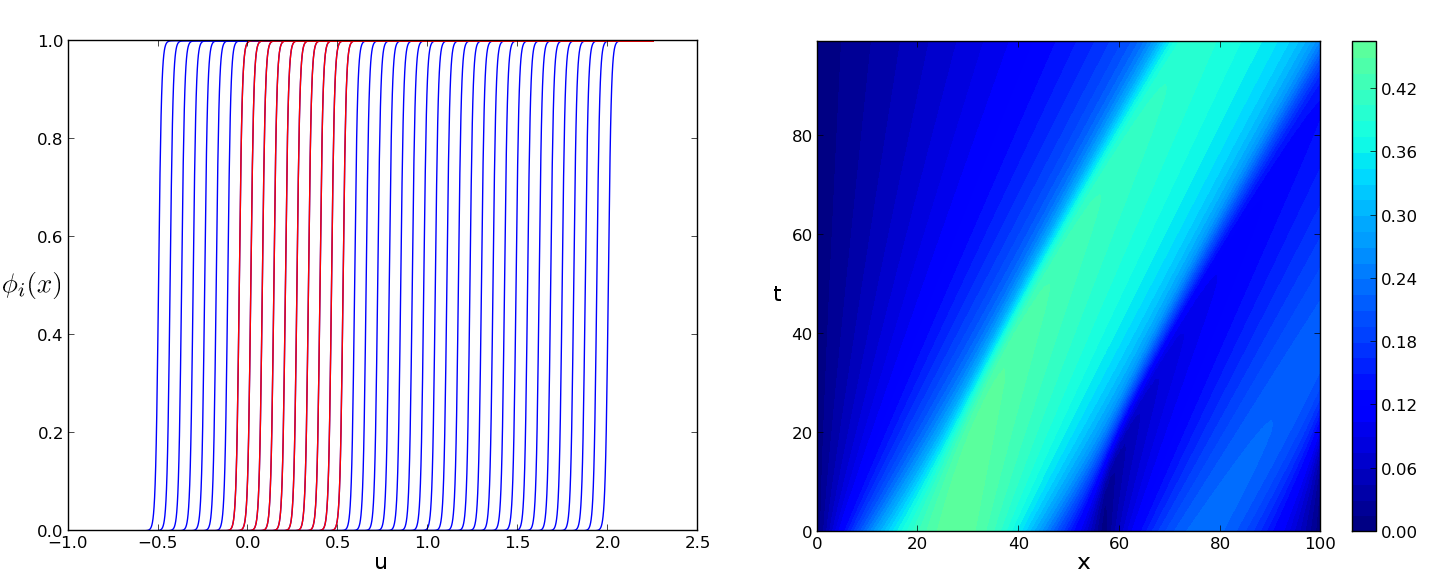
\includegraphics[height=5cm]{all.png}
    \caption{Basis selection using Lasso. The figure on the right side shows
    the primal model's solution $u(t,x)$. The figure on the left side shows all
    candidate bases. The selected bases are colored red. Notice how the selected
    bases correspond to the colorbar of the primal model solution.}
    \label{fig:basis_selection_1}
    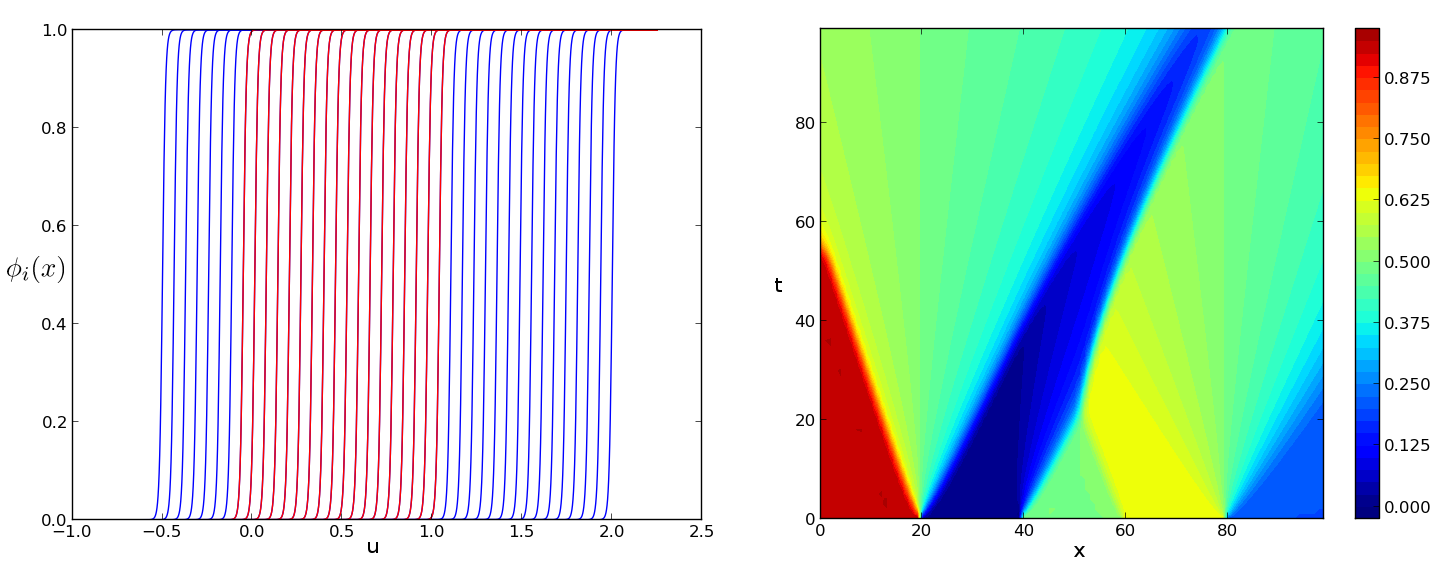
\includegraphics[height=5cm]{all2.png}
    \caption{Basis selection with a different $u(t,x)$. Notice
    how selected bases depend on the primal model solution.}
    \label{fig:basis_selection_2}
\end{center}
\end{figure}

\subsection{Future work}
The sections above provide a framework to infer the twin model for time-dependent primal models 
with unknown flux functions. However, there are three issues to investigate.\\

\noindent Firstly, we need to extend the theory to more general problems.
We should investigate twin models with unknown source term, and
twin models with both unknown source term and flux function.
Besides, we need to study time-independent (steady state) twin model.
If we think of using time \emph{dependent} twin model to match a video (time-space solution),
then we use time \emph{independent} twin model to match an image (space-only solution).\\

\noindent Secondly, we need to explore the weighting scheme used in Eqn\eqref{minimizer twin model}.
Loosely speaking, choosing $w=1$ is equivalent to setting a uniform sample weight, where each `sample'
corresponds to the solution at a spatial and time grid point.
By using a variable $w$, we should be able to fine tune the twin model accuracy at different locations
in the excited domain $\mathcal{E}$. For example, should we assign a larger $w$
for regions with sparser samples? Or should we assign a larger $w$ for regions where
more interesting physics happen (e.g. around a shock wave)?
The weighting scheme may be ad hoc, but can possibly 
improve the twin model's accuracy for specific numerical examples.\\


\noindent Thirdly, in section \ref{adaptive}, we discussed twin model with adaptive structure.
The proposed approach constructs a \emph{fixed} candidate basis library, then selects a subset of basis
from the library.
However, the cardinality of the basis library can be high for flux functions with a large number
of inputs, for example $F(u_1,\cdots,u_n)$ with a large $n$. Besides, the proposed basis
library may be inefficient to represent flux of the form $F(\mathbf{w}^T \mathbf{u})$, where 
$\mathbf{w}$ is
a constant vector. Although $F(\mathbf{w}^T \mathbf{u})$ can be reduced to a univariate
function by a change of variable $u^* = \mathbf{w}^T \mathbf{u} \in\mathbb{R}$, 
the fixed basis library 
can not take advantage of it.
Therefore, the twin model method may be improved by choosing 
a set of basis from an \emph{non-fixed} basis library.
A literature survey is required 
to determine the most appropriate method to use.

\newpage
\section{Optimization with twin model}
\noindent In chapter \ref{gradient_surrogate},
we developed twin model as a physics-based surrogate method.
How should we leverage this surrogate to facilitate optimizations based on gray-box simulations?
In this chapter, we answer this question by developing a provably convergent optimization scheme.
We also demonstrate our method's superiority for optimization with high-dimensional controls.\\

\subsection{Motivation of the Bayesian approach}
We are interested in optimization problems of the following form
\begin{equation}\begin{split}
    \min_{c\in\mathcal{C}} & J(u,c)\\
    \textrm{where}\; u\; \textrm{satisfies}& \;\; \mathcal{R}(u,c) = 0\\
    \textrm{subject to} \; \mathcal{C} & = \left\{\left. c\in\mathbb{R}^d\right| 
    A c\le b, V(c)\le 0\right\}
\end{split}\label{general opt}
\end{equation}
where $u(t,\mathbf{x})\in\mathbb{R}\,, t\in[0,T], \,x\in\Omega$
is the space-time solution of a PDE abstracted as
$\mathcal{R}$, with given initial and boundary conditions.
The controls are $c\in\mathbb{R}^d$. 
There are $l$ linear constraints defined by $A\in\mathbb{R}^{l\times d}$ and $b\in\mathbb{R}^{l}$
and $s$ nonlinear constraints defined by $V(c)\in \mathbb{R}^s$. 
These linear and nonlinear constraints define a feasible region 
$\mathcal{C}\subseteq \mathbb{R}^d$. The evaluation of $J$ for a given $c$ requires
solving the PDE $\mathcal{R}(u,c)=0$ which can be computational costly, such
as large eddy simulation (LES) \cite{LES, LES oldest} 
and direct numerical simulation (DNS) \cite{DNS} in  
aerodynamic design problems.
In addition to expensive evaluations of $J$, the evaluations of
nonlinear constraints $V(c)$ can be similarly expensive. For example, 
in airfoil design we may aim at reducing drag while keeping lift 
above a threshold value \cite{constraint lift}. Evaluating the lift of a given design
requires simulating the flow. Besides, we consider the PDE and its solver 
as a gray-box. Finally, we consider controls of high dimension, i.e. $d\gg 1$.\\

\noindent We start with optimization problem Eqn\eqref{general opt} with feasible region
$\mathcal{C}=\mathbb{R}^d$ for simplicity.
There are already many methods that deal with such optimizations. 
But as mentioned in section \ref{gradfree_gradbased}, these methods are not suitable
for our problem because they either require adjoint-based gradient of the PDE solver, 
or suffer the curse of dimensionality. Can we utilize the twin model together
with the primal model, and develop an optimization scheme that addresses these challenges?\\

\noindent The question fits naturally into a \emph{multifidelity optimization (MFO)} framework.
MFO performs optimization with multiple models ranging from
low-fidelity to high-fidelity. Conventionally, low-fidelity models are cheaper to solve, but yield
results with less credibility; high-fidelity models are more credible, but more expensive
to solve. MFO balances computation investments between high-fidelity and low-fidelity models
in order to reach optimum with overall less computation cost.
In our problem, the primal model can be considered as high-fidelity model, and the twin model
can be considered as low-fidelity model.\\

\noindent MFO methods can take various flavors.
For example, a MFO method can be as simple as a two-stage optimization \cite{MFO: two stage}. 
In the first stage it optimizes with the low-fidelity model only. In the second stage
it optimizes with the high-fidelity model only, using the first stage optimum as the initial guess.
However, we are only interested in \emph{provably convergent} MFO methods.
Based on our literature review, there are three types of such methods:
\emph{pattern search MFO}, \emph{trust region MFO}, and \emph{Bayesian calibration MFO}.
Each type can be viewed as 
extensions to their \emph{single-fidelity} versions respectively,
i.e. \emph{pattern search methods}, \emph{trust region methods}, and \emph{Bayesian 
calibration methods}. In the following let's review these methods and 
their corresponding MFO methods.\\

\noindent In \emph{pattern search methods}, the objective function $J$ is evaluated at a set of
trial points, called `mesh', adjacent to the current best $c$ in the design space. This
step is called `poll step'.
If improvement in $J$ is obtained, the current best $c$ is updated; otherwise, the mesh size
is shrinked. 
These steps are iterated until convergence \cite{Pattern Search Convergence}.
Pattern search methods can takes advantage of low-fidelity models to reduce computation cost,
hereby \emph{pattern search MFO}.
It searches for improved design 
points using low-fidelity model before deciding whether to perform a poll step on
the high-fidelity model \cite{Pattern Search Convergence MFO}.
However, each poll step requires order $d$ high-fidelity model evaluations, which can
be too expensive to afford in our problem settings.\\

\noindent In \emph{trust region methods}, a functional surrogate is firstly constructed from
evaluations of $J$, then the surrogate is minimized within a trust-region to generate
a candidate design point. Depending on the availability of $\frac{\partial J}{\partial c}$,
the functional surrogate can either use the gradient information \cite{inexactgradient1},
or not use the gradient information \cite{jones1998, trustregionconn, trustregionwild}.
When a low-fidelity model exists,
the functional surrogate of $J$ can be replaced by the low-fidelity model, hereby
\emph{trust region MFO} \cite{simplified physics, coarse discretization}.
To improve MFO performance and guarantee convergence,
researchers have proposed using functional surrogates to account for 
the discrepancy $\Delta J = J_{high} - J_{low}$
between high- and low- fidelity models within the trust region
\cite{andrewras, andrew thesis}. However, there are two problems with trust region MFO.
Firstly, the convergence proof of such methods requires
a condition called \emph{fully-linearity} \cite{trustregionconn}. The fully-linearity
condition bounds the deviation of $\frac{dJ}{dc}$ between the high- and low-
fidelity models within the trust region. As mentioned in
chapter \ref{intro}, it can be hard to obtain the gradient from the primal model.
Therefore, it can be hard to certify fully-linearity and to support 
the convergence proof.
Secondly, as mentioned in section \ref{review surrogate methods}, constructing
a functional surrogate for $\Delta J$ may require a large amount
of low- and high- fidelity model evaluations when $d$ is large.
Therefore, trust region MFO is not suitable for our problem settings too.\\

\noindent In \emph{Bayesian optimization methods}, $J$ as a function of $c$
is assumed to be an unknown sample from a \emph{stochastic process (SP)}. 
Bayesian optimization starts from a prior distribution of $J$, and
updates its posterior as new samplings of $J(c)$ arrive.
Then it constructs an \emph{acquisition function} $\rho: \mathcal{C}\mapsto \mathbb{R}\;
,\; c\rightarrow \rho(c)$ from the posterior, which measures
the expected utility of investing the next sample at $c$.
Finally, we choose the next sample as the maximizer of the acquisition function.
Bayesian optimization iterates over the posterior-update step and the 
acquisition-function-maximization step until convergence.

1. all information, optimal
2. incompatible source of data
3. 

The SP can vary depending
on its \emph{covariance} (also called \emph{kernel}).
Among the most popular choices are Gaussian kernels \cite{KennedyOhagan1}
and Matern kernels \cite{practicalBayesianopt}.


Bayesian calibration \cite{convergenceBayesian, KennedyOhagan1}
Bayesian calibration with gradient \cite{gradient kriging surrogate}
Kriging and cokriging \cite{kriging, cokriging}
similar to Krigin whose acquisition is a special function, just the mean
\cite{kriging functional surrogate}, also grad cokriging 
\cite{adjoint gradient cokriging without MLE}

 However, it is worth noting that the twin model
may not be cheap to solve. Constructing a twin model requires an optimization itself 
(Eqn\eqref{objective twin model} or Eqn\eqref{objective twin model steady}).
Therefore, the MFO with twin model may not fit into the conventional ideology:
`expensive high fidelity model, cheap low fidelity model'.
If the twin model is expensive, why should we use it?

2. Training twin model costly (evaluate a PDE and ajdoint, iteratively nonlinear solve for training)
   low fidelity is expensive too. 
3. Gradient, proof
   \begin{figure}[H]
       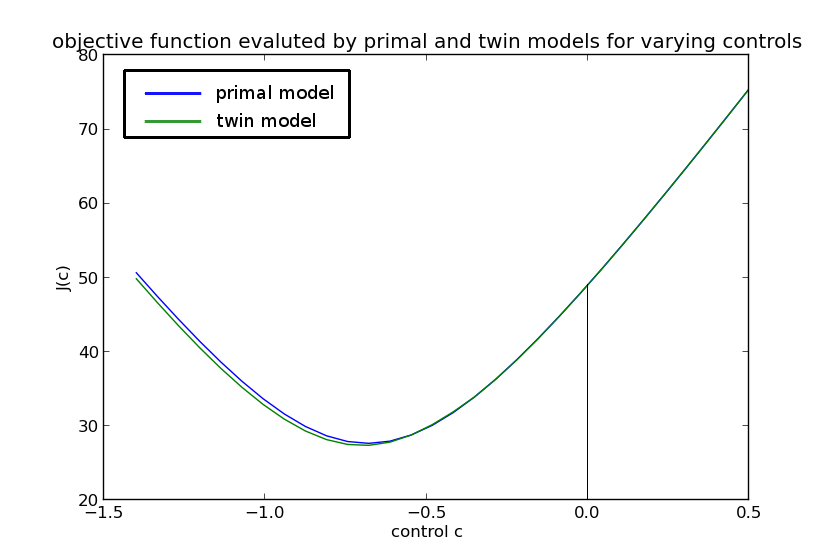
\includegraphics[width=4cm]{J_twin_vs_primal.png}
   \end{figure}
3. Bayesian optimization \cite{Mockus Bayesian opt, practicalBayesianopt}
   Desirable to spend computation to making better choices about where to seek the best next sample.
   Also, good for fusion data of different types (cokriging).
   acquisition function EI, UCB(no convergence proof)


\subsection{Bayesian modeling of the primal and twin models}
\label{bayesian_model}
Stochastic process model. The simulation output is modeled as a stochastic process
DACE(Design and Analysis of Computer Experiments Kennedy Ohagan Jones 1998)
$$
y(x^{(i)}) = \mu + \epsilon(x^{(i)})
$$
where $\mu$ is the mean of the stochastic process. $\epsilon(x^{(i)})$ is ...
Concentrated likelihood function



\subsection{Optimization using the posterior of the objective function}
\label{bayesian_opt}
why not mu+k*sigma, counter example of no convergence.
Sampling next design point as a design of experiment problem.
Why use Bayesian optimization (compare to gradient-descent, and gradient-free). Proven convergence
(I'm not able to prove with gradient)
Stochastic process modeling of model.
Expected improvement
Use gradient information: cascading posterior
Error estimate (covariance) of estimated gradient
Example:
Qudratic high-dimensional analysis (Convergence rate change with dimension)
\subsection{Optimization constraints}
\label{constraints}
Geometric inequalities, easy
costly to evaluate inqualities, feasible region, hard
constraint c(x) evaluated by primal, and dcdx at twin, indicator
\cite{constraint Bayesian Opt}
Another method is Lagrangian, convert to unconstraint (different from Lagrange multipliers). 
(see wiki)
penalty method, augmented Lagrange method
Equality nonlinear constraints 
\cite{equality nonlinear constraint trust region opt}
Extend to inequality nonlinear constraint \cite{coarse discretization}

\subsection{Complete algorithm}
\label{complete algo}

\subsection{Twin model validation}
If primal model uses not accurate solver, if dependence is not local so no PDE can be written,
like integral equation
Laplace rho = phi is impossible (Helmholtz equation)
that is because knowledge of twin model basic structure is wrong.
Report if twin model fails.


\section{Application to a high-fidelity flow simulator}
\label{examples}
High-fidelity turbulence simulation and RANS twin model


\begin{appendices}
    \section{Proof of theorem \ref{theorem: 1}: global-local error}
    \label{appendix 1}
    \emph{Proof:} Consider a primal model and a twin model solving
    for the space-time solution $u$ and $\tilde{u}$ on the same
    time grid $\{t_0=0,t_1,\cdots, t_n=T\}$. The solutions at timestep $t_i$
    are $u_i$ and $\tilde{u}_{i}$. Both simulations 
    starts from the same initial condition $u_0$. Define the mapping
    of the primal model 
    \begin{equation}
        H:\, \mathbb{R}^n\mapsto\mathbb{R}^n,\, u^i\rightarrow Hu^i = u^{i+1}\,,
        \quad i=1,\cdots, n
    \end{equation}
    and the mapping of the twin model
    \begin{equation}
        G:\, \mathbb{R}^n\mapsto\mathbb{R}^n,\, \tilde{u}^i\rightarrow 
        G\tilde{u}^i = \tilde{u}^{i+1}\,,\quad i=1,\cdots, n
    \end{equation}
    $G$ and $H$ are linear or nonlinear mappings.
    We illustrate these mappings in Fig \ref{fig:sketch}.
    \begin{figure}[H]\begin{center}
        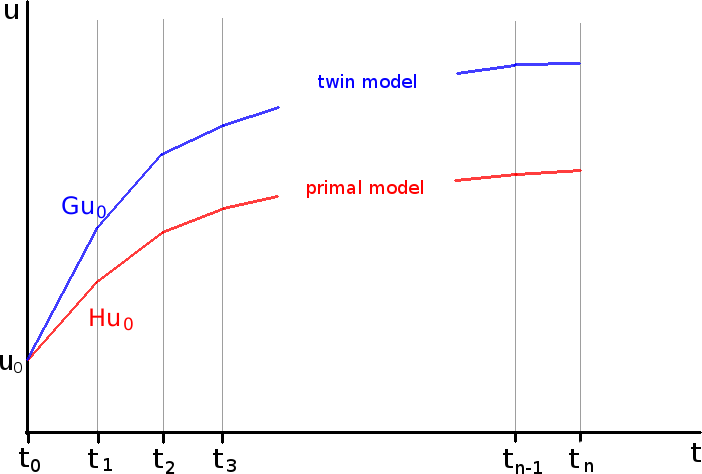
\includegraphics[height=5cm]{sketch.png}
        \caption{Trajectories of the primal model and the twin model. 
                 $H$ and $G$ are their timestep-wise mapping functions.}
        \label{fig:sketch}
    \end{center}\end{figure}
    \noindent The global error is
    \begin{equation}
        Err_G = \frac{1}{n\Delta t}\left\{ \|(G^n - H^n) u_0\| + \|(G^{n-1}-H^{n-1})u_0\|
        +\cdots+\|(G^1-H^1)u_0\| \right\}
        \label{global error}
    \end{equation}
    The local error is
    \begin{equation}
        Err_L = \frac{1}{n\Delta t} \left\{
            \|\left(GH^{n-1} - H^{n}\right)u_0\| +  
            \|\left(GH^{n-2} - H^{n-1}\right)u_0\| + \cdots +
            \|\left(G^1-H^1\right)u_0\|
        \right\}
        \label{local error}
    \end{equation}
    Using the equality
    \begin{equation}
        G^i-H^i = (G^i-G^{i-1}H) + (G^{i-1}H - G^{i-2}H^2) + \cdots + (GH^{i-1}-H^i)\,,\quad
        i\in \mathbb{Z}^+\,,
    \end{equation}
    we derive from Eqn\eqref{global error}
    \begin{equation}
        Err_G \le \frac{1}{n\Delta t}
        \left\{\begin{split}
            \|(G^{n-1} G - G^{n-1}H)u_0\| &+ \|(G^{n-2}GH - G^{n-2}H^2)u_0\|&+\cdots
            &+ \|(GH^{n-1} - H^{n})u_0\|\\
            &+\|(G^{n-2} G - G^{n-2}H)u_0\| &+ \cdots 
            &+ \|(GH^{n-2} - H^{n-1})u_0\|\\
            &\ddots&& \vdots\\
            &&& + \|(G - H)u_0\|
        \end{split}
        \right\}
        \label{expansion global error}
    \end{equation}
    Using Eqn\eqref{expansion global error} and Eqn\eqref{local error}, we get
    \begin{equation}
        Err_G - Err_L \le 
        \frac{1}{n\Delta t}
        \left\{\begin{split}
            \|(G^{n-1} G - G^{n-1}H)u_0\| &+ \|(G^{n-2}GH - G^{n-2}H^2)u_0\|&+\cdots
            &+ \|(GGH^{n-2} - G H^{n-1})u_0\|\\
            &+\|(G^{n-2} G - G^{n-2}H)u_0\| &+ \cdots 
            &+ \|(GGH^{n-3} - G H^{n-2})u_0\|\\
            &\ddots&& \vdots\\
            &&& + \|(G G - G H)u_0\|
        \end{split}
        \right\}
        \label{error diff}
    \end{equation}
    Apply our assumption
    \begin{equation}
        \left\| Gx - Gy \right\| \le \alpha \|x-y\|
    \end{equation}
    and its implication
    \begin{equation}
        \left\|G^i x - G^i y\right\| \le \alpha^i \|x-y\|\,, \quad i\in \mathbb{Z}^+
    \end{equation}
    to Eqn\eqref{error diff}, we get
    \begin{equation}
        Err_G - Err_L \le 
        \frac{1}{n\Delta t}
        \left\{\begin{split}
            \alpha^{n-1}\|(G - H)u_0\| &+ \alpha^{n-2}\|(GH - H^2)u_0\|&+\cdots
            &+ \alpha\|(GH^{n-2} - H^{n-1})u_0\|\\
            &+\alpha^{n-2}\|( G - H)u_0\| &+ \cdots 
            &+ \alpha\|(GH^{n-3} - H^{n-2})u_0\|\\
            &\ddots&& \vdots\\
            &&& + \alpha\|(G - H)u_0\|
        \end{split}
        \right\}
        \label{error diff}
    \end{equation}
    Reorder the summation, we get
    \begin{equation}
        Err_G - Err_L \le 
        \frac{1}{n\Delta t}
        \left\{\begin{split}
            \alpha^{n-1}\|(G - H)u_0\| &+ \alpha^{n-2}\|(G - H)u_0\|&+\cdots
            &+ \alpha\|(G - H)u_0\|\\
            &+\alpha^{n-2}\|( GH - H^2)u_0\| &+ \cdots 
            &+ \alpha\|(GH - H^{2})u_0\|\\
            &\ddots&& \vdots\\
            &&& + \alpha\|(GH^{n-2} - H^{n-1})u_0\|
        \end{split}
        \right\}
        \label{error diff 2}
    \end{equation}
    Therefore, from Eqn\eqref{error diff 2} and Eqn\eqref{local error}, we get
    \begin{equation}
        Err_G \le (1+\alpha+\cdots+\alpha^{n-1}) Err_L\,.
    \end{equation}
    If $|\alpha|$ is strictly less than $1$, 
    \begin{equation}
        Err_G \le \frac{1}{1-\alpha} Err_L\,,
    \end{equation}
    which completes the proof.$\hfill\Box$

    \section{Proof of theorem \ref{theorem: 2}: gradient of twin model}
    What to prove: If the twin model flux and rhs is close to the primal model,
    then the gradients are close. Intermediate step, the adjoint state are close.
    Consider objective function $\int_t\int_{\Omega} J(u,c)$.
    The adjoint satisfies
    \begin{equation}
        \frac{\partial \lambda}{\partial t} + \nabla F(u)\cdot \nabla\lambda
        = \frac{\partial J}{\partial u} - \frac{\partial q}{\partial u}\lambda
    \end{equation}
    with $\lambda(T) = 0$ and $\lambda\big|_{\partial \Omega} = 0$.\\
    Need to show: if $\|F_1-F_2\|$ and $\|q_1-q_2\|$ are bounded, then
    $\|\lambda_1-\lambda_2\|$ is bounded.
    \section{Proof of theorem \ref{theorem: 3}: optimization convergence}
\end{appendices}

\begin{thebibliography}{9}
\bibitem{hanmaster} 
Han Chen.
"Blackbox stencil interpolation method for model reduction"
Master thesis, 2012
 

\bibitem{andrewras}
March, Andrew, Karen Willcox, and Qiqi Wang. 
"Gradient-based multifidelity optimisation for aircraft design using Bayesian model calibration." 
Aeronautical Journal 115.1174 (2011): 729.

\bibitem{jones1998}
Jones, Donald R., Matthias Schonlau, and William J. Welch. 
"Efficient global optimization of expensive black-box functions." 
Journal of Global optimization 13.4 (1998): 455-492.

\bibitem{convergenceBayesian}
Bull, Adam D. 
"Convergence rates of efficient global optimization algorithms." 
The Journal of Machine Learning Research 12 (2011): 2879-2904.

\bibitem{NARMAXbook}
Stephen A Billings.
"Nonlinear System Identification, NARMAX methods in time, frequency and spatial-temporal domains"
ISBN:978-1-119-94359-4, 2013

\bibitem{practicalBayesianopt}
Snoek, Jasper, Hugo Larochelle, and Ryan P. Adams. 
"Practical Bayesian optimization of machine learning algorithms." 
Advances in Neural Information Processing Systems. 2012.

\bibitem{KennedyOhagan1}
Kennedy, Marc C., and Anthony O'Hagan. 
"Predicting the output from a complex computer code when fast approximations are available." 
Biometrika 87.1 (2000): 1-13.

\bibitem{inexactgradient1}
Carter, Richard G. 
"Numerical experience with a class of algorithms for nonlinear optimization using inexact function and gradient information." 
SIAM Journal on Scientific Computing 14.2 (1993): 368-388.

\bibitem{inexactnewton1}
Dembo, Ron S., Stanley C. Eisenstat, and Trond Steihaug. 
"Inexact newton methods." 
SIAM Journal on Numerical analysis 19.2 (1982): 400-408.

\bibitem{trustregionconn}
Conn, Andrew R., Katya Scheinberg, and Luís N. Vicente. 
"Global convergence of general derivative-free trust-region algorithms to first-and second-order critical points." 
SIAM Journal on Optimization 20.1 (2009): 387-415.

\bibitem{trustregionwild}
Wild, Stefan M., and Christine Shoemaker. 
"Global convergence of radial basis function trust-region algorithms for derivative-free optimization." 
SIAM Review 55.2 (2013): 349-371.

\bibitem{kriging}
G.M. Matheron,
"Principles of geostatistics".
Economic Geology 58.8 (1963): 1246-1266

\bibitem{cokriging}
Goovaerts, Pierre. 
"Ordinary cokriging revisited." 
Mathematical Geology 30.1 (1998): 21-42.

\bibitem{bishopbook}
Christopher M. Bishop
Pattern recognition and machine learning
ISBN: 978-0387310732. 2007

\bibitem{SarmaEKF}
Sarma, Pallav, LJ Durlofsky, K Aziz, WH Chen. 
"Efficient real-time reservoir management using adjoint-based optimal control and model updating." 
Computational Geosciences 10.1 (2006): 3-36.

\bibitem{gradfreereview}
Rios, Luis Miguel, and Nikolaos V. Sahinidis. 
"Derivative-free optimization: A review of algorithms and comparison of software implementations." 
Journal of Global Optimization 56.3 (2013): 1247-1293.

\bibitem{dynamicprogramming}
Powell, Warren B.
"Approximate Dynamic Programming: Solving the curses of dimensionality".
Vol. 703. John Wiley \& Sons, 2007.

\bibitem{quasiNewton}
Dennis, Jr, John E., and Jorge J. Moré. 
"Quasi-Newton methods, motivation and theory." 
SIAM review 19.1 (1977): 46-89.

\bibitem{adjoint}
Plessix, R-E. 
"A review of the adjoint-state method for computing the gradient of a functional with geophysical applications." 
Geophysical Journal International 167.2 (2006): 495-503.

\bibitem{cont discretize adjoint}
Nadarajah, Siva, and Antony Jameson. 
"A comparison of the continuous and discrete adjoint approach to automatic aerodynamic optimization." 
AIAA paper 667 (2000): 2000.

\bibitem{automaticdiff}
A Griewank, GF Corliss
Automatic differentiation of algorithms: theory, implementation, and application.
Defense Technical Information Center, 1992.

\bibitem{reservoir simulation book}
Zhangxin Chen
"Reservoir Simulation: Mathematical Techniques in Oil Recovery"
Society for Industrial and Applied Mathematics, ISBN 0898716403, 2007

\bibitem{wavelet mallat}
Mallat, Stephane G. 
"A theory for multiresolution signal decomposition: the wavelet representation." 
Pattern Analysis and Machine Intelligence, IEEE Transactions on 11.7 (1989): 674-693.

\bibitem{Bayopt converge 2}
Vazquez, Emmanuel, and Julien Bect. 
"Convergence properties of the expected improvement algorithm with fixed mean and covariance functions." 
Journal of Statistical Planning and inference 140.11 (2010): 3088-3095.

\bibitem{Buckley Leverett}
S.E. Buckley and M.C. Leverett
"Mechanism of fluid displacement in sands."
Transactions of the AIME 146 (1942): 107-116

\bibitem{Reservoir Simulation Book}
Chen, Zhangxin, Guanren Huan, and Yuanle Ma. 
"Computational methods for multiphase flows in porous media."
Vol. 2. Siam, 2006.

\bibitem{Boyd optimization}
Stephen Boyd and Lieven Vandenberghe
"Convex Optimization"
Cambridge University Press, 2004

\bibitem{Sigmoid Approximation}
G. Cybenko
"Approximation by superpositions of a sigmoid function"
Mathematics of control, signals and systems 2.4 (1989): 303-314

\bibitem{haar}
Alfred Haar
"On the theory of orthogonal function systems"
Mathematische Annalen 69 (1910): 331-371

\bibitem{Analytic Meyer}
V.VV. Vermehren, H.M. de Oliveira
"Close expressions for Meyer wavelet and scale function"
arXiv:1502.00161 [stat.ME]

\bibitem{Opt Koziel Book}
Slawomir Koziel, Xin-She Yang
"Computational optimization, methods and algorithms"
Springer Berlin Heidelberg, 2011

\bibitem{Surrogate based analysis and optimization}
N.V. Queipo, R.T. Haftka, W. Shyy, T. Goel, R. Vaidynathan, P.K Tucker
"Surrogate-based analysis and optimization"
Progress in Aerospace Sciences 41 (2005): 1-28

\bibitem{Space mapping 1}
T.D. Robinson, M.S. Eldred, K.E. Willcox, R. Haimes
"Surrogate-based optimization using multifidelity models with variable 
parameterization and corrected space mapping"
AIAA Journal 46 (2008): 2814-2822

\bibitem{Space mapping 2}
Mohamed H. Bakr, John W. Bandler
"An introduction to the space mapping technique"
Optimization and Engineering 2 (2011): 369-384

\bibitem{simplified physics}
N.M. Alexandrov, E.J. Nielsen, R.M. Lewis, W.K. Anderson
"First-Order Model Management with Variable-Fidelity Physics 
Applied to Multi-Element Airfoil Optimization"
8th AIAA Symposium on Multidisciplinary Design and Optimization (2000)

\bibitem{equality nonlinear constraint trust region opt}
Conn, Andrew R., Nicholas IM Gould, and Philippe Toint. 
"A globally convergent augmented Lagrangian algorithm for optimization with general constraints and simple bounds."
SIAM Journal on Numerical Analysis 28.2 (1991): 545-572.

\bibitem{coarse discretization}
N.M. Alexandrov, R.M. Lewis, C.R. Gumbert, L.L. Green, P.A. Newmann
"Optimization with Variable-Fidelity Models Applied to Wing Design"
38th Aerospace Sciences Meeting (2000)

\bibitem{gradient kriging surrogate}
Han Zhong-Hua, Stefan Görtz, Ralf Zimmermann
"Improving variable-fidelity surrogate modeling via gradient-enhanced kriging and a generalized hybrid bridge function."
Aerospace Science and Technology 25.1 (2013): 177-189.

\bibitem{poly functional surrogate}
Gary G. Wang, S. Shan
"Review of metamodeling techniques in support of engineering design optimization."
Journal of Mechanical Design 129.4 (2007): 370-380.

\bibitem{kriging functional surrogate}
Shinkyu Jeong, Mitsuhiro Murayama, Kazuomi Yamamoto
"Efficient optimization design method using kriging model" 
Journal of aircraft 42.2 (2005): 413-420.

\bibitem{ann functional surrogate}
Nestor V. Queipo, Javier V. Goicochea, Salvador Pintos. 
"Surrogate modeling-based optimization of SAGD processes." 
Journal of Petroleum Science and Engineering 35.1 (2002): 83-93.

\bibitem{adjoint gradient cokriging without MLE}
Hyoung-Seog Chung, Juan J. Alonso. 
"Using gradients to construct cokriging approximation models for high-dimensional design optimization problems." 
AIAA paper 317 (2002): 14-17.

\bibitem{survey of high dimensional blackbox optimization}
Songqing Shan, G. Gary Wang. 
"Survey of modeling and optimization strategies to solve high-dimensional design problems with computationally-expensive black-box functions." 
Structural and Multidisciplinary Optimization 41.2 (2010): 219-241.

\bibitem{review of black-box modeling}
Jonas Sjöberg et al.
"Nonlinear black-box modeling in system identification: a unified overview." 
Automatica 31.12 (1995): 1691-1724.

\bibitem{dimensional reduction}
Laurens JP van der Maaten, Eric O. Postma, H. Jaap van den Herik
"Dimensionality reduction: A comparative review." 
Journal of Machine Learning Research 10.1-41 (2009): 66-71.

\bibitem{decomposition}
T.R. Browning
"Applying the design structure matrix to system decomposition and integration problems: a review
 and new directions"
IEEE Trans Eng Manage 48.3 (2001): 292-306

\bibitem{variable selection}
Raymond H. Myers, Douglas C. Montgomery, Christine M. Anderson-Cook
"Response surface methodology: process and product optimization using designed experiments"
Vol. 705. John Wiley and Sons, 2009

\bibitem{thin airfoil}
Ira H. Abbott, E. Albert Von Doenhoff
"Theory of wing sections"
Dover Publications Inc., Section 4.2 (1959)

\bibitem{turbulent modeling R high}
Tsan-Hsing Shih, et al. 
"A new k-ϵ eddy viscosity model for high reynolds number turbulent flows" 
Computers and Fluids 24.3 (1995): 227-238.

\bibitem{turbulent modeling R low}
Virendra C. Patel, Wolfgang Rodi, and Georg Scheuerer
"Turbulence models for near-wall and low Reynolds number flows-a review"
AIAA journal 23.9 (1985): 1308-1319

\bibitem{NP hard}
Toby S. Cubitt, Jens Eisert, Michael M. Wolf
"Extracting dynamical equations from experimental data is NP hard"
Physical review letters 108.12 (2012): 120503

\bibitem{Hamilton Fluid Dynamics}
Rick Salmon 
"Hamiltonian fluid mechanics"
Annual review of fluid mechanics 20.1 (1988): 225-256

\bibitem{numerical schemes for hyperbolic equation review}
Randall J. LaVeque
"Finite volume methods for hyperbolic problems"
Vol. 31. Cambridge university press, 2002

\bibitem{SI old}
Pieter Eykhoff
"System identification, parameter and system estimation"
John Wiley and Sons, 1974

\bibitem{piecewise linear}
S.A. Billings, W.S.F Voon
"Piecewise linear identification of non-linear system"
International Journal of Control, 46.1 (1987): 215-235

\bibitem{volterra 1}
Georgios B. Giannakis, Erchin Serpedin
"A bibliography on nonlinear system identification"
Signal Processing 81.3 (2001): 533-580

\bibitem{volterra 2}
M.J. Korenberg, I.W. Hunter
"The Identification of Nonlinear Biological Systems: Volterra Kernel Approaches"
Annals Biomedical Engineering 24.2 (1996): 250-268

\bibitem{cross correlation}
Julian Jakob Bussgang
"Crosscorrelation functions of amplitude-distorted Gaussian signals" 
(1952)

\bibitem{feedback linear}
C.P. Kwong, C. F. Chen
"Linear feedback system identification via block-pulse functions"
International Journal of Systems Science 12.5 (1981): 635-642

\bibitem{billings 1981}
S.A. Billings, I.J. Leontaritis
"Identification of nonlinear systems using parametric estimation techniques"
Proceedings of the IEE Conference on Control and its Application, Warwick, UK, pp.183-187

\bibitem{ANN SI}
Sheng Chen, S. A. Billings, P. M. Grant
"Non-linear system identification using neural networks" 
International journal of control 51.6 (1990): 1191-1214

\bibitem{Wavelet SI}
Stephen A. Billings, Hua-Liang Wei
"A new class of wavelet networks for nonlinear system identification."
Neural Networks, IEEE Transactions on 16.4 (2005): 862-874.

\bibitem{correlation model validation}
S. A. Billings, W. S. F. Voon
"Correlation based model validity tests for non-linear models"
International Journal of Control 44.1 (1986): 235-244.

\bibitem{Dijkema book}
Tammo Jan. Dijkema
"Adaptive tensor product wavelet methods for solving PDEs"
PhD thesis, Utrecht University (2009)

\bibitem{simple opt}
Ismail Kucuk,  Ibrahim Sadek
"An efficient computational method for the optimal control problem for the Burgers equation." 
Mathematical and computer modelling 44.11 (2006): 973-982.

\bibitem{numpad}
Qiqi Wang,
Numpad package,
https://github.com/qiqi/numpad.git

\bibitem{sklearn}
Scikit-learn package,
https://github.com/scikit-learn/scikit-learn.git

\bibitem{nlopt}
Steven G. Johnson,
The NLopt nonlinear-optimization package, 
http://ab-initio.mit.edu/nlopt

\bibitem{Quasi-Newton Review}
John E. Dennis, Jorge J. Moré.
"Quasi-Newton methods, motivation and theory." SIAM review 19.1 (1977): 46-89.

\bibitem{Eric master thesis}
Eric Alexander. Dow,
"Quantification of structural uncertainties in RANS turbulence models."
Dissertation, Massachusetts Institute of Technology, 2011.

\bibitem{LBFGS}
J. Nocedal.
"Updating quasi-Newton matrices with limited storage"
Mathematics of Computation, 35 (1980): 773-782

\bibitem{review dimensional reduction}
Van der Maaten, Laurens JP, Eric O. Postma, and H. Jaap van den Herik. 
"Dimensionality reduction: A comparative review." 
Journal of Machine Learning Research 10.1-41 (2009): 66-71.

\bibitem{review variable selection}
Havi, Ron, and George H. John. 
"Wrappers for feature subset selection."
Artificial intelligence 97.1 (1997): 273-324.

\bibitem{Billing feature selection}
Wei, Hua-Liang, and Stephen A. Billings. 
"Feature subset selection and ranking for data dimensionality reduction." 
Pattern Analysis and Machine Intelligence, IEEE Transactions on 29.1 (2007): 162-166.

\bibitem{PCA review}
Jolliffe, Ian. Principal component analysis. John Wiley and Sons, Ltd, 2002.

\bibitem{constraint Bayesian Opt}
Gardner, Jacob, et al. 
"Bayesian optimization with inequality constraints."
Proceedings of The 31st International Conference on Machine Learning. 2014.

\bibitem{Lasso variable selection}
Tibshirani, Robert. 
"Regression shrinkage and selection via the lasso." 
Journal of the Royal Statistical Society. Series B (Methodological) (1996): 267-288.

\bibitem{Critical review of variable selection}
Dziak, John, Runze Li, and Linda Collins. 
"Critical review and comparison of variable selection procedures for linear regression (Technical report)." (2005).

\bibitem{stepwise variable selection}
Derksen, Shelley, and H. J. Keselman. 
"Backward, forward and stepwise automated subset selection algorithms: Frequency of obtaining authentic and noise variables." 
British Journal of Mathematical and Statistical Psychology 45.2 (1992): 265-282.

\bibitem{Elastic net variable selection}
Zou, Hui, and Trevor Hastie. 
"Regularization and variable selection via the elastic net." 
Journal of the Royal Statistical Society: Series B (Statistical Methodology) 67.2 (2005): 301-320.

\bibitem{AIC}
Stone, Mervyn. 
"An asymptotic equivalence of choice of model by cross-validation and Akaike's criterion." 
Journal of the Royal Statistical Society. Series B (Methodological) (1977): 44-47.

\bibitem{BIC}
Schwarz, Gideon. 
"Estimating the dimension of a model." 
The annals of statistics 6.2 (1978): 461-464.

\bibitem{Mockus Bayesian opt}
J Mockus, V Tiesis, and A Zilinskas
"The application of Bayesian methods for seeking the extreme."
Towards Global Optimization, 2 (1978): 117-129

\bibitem{MFO: two stage}
Choi, Seongim, Juan J. Alonso, and Ilan M. Kroo. 
"Two-level multifidelity design optimization studies for supersonic jets." 
Journal of Aircraft 46.3 (2009): 776-790.

\bibitem{MFO: bayesian discrepancy aerodynamics}

\bibitem{MFO: trust region acdl}
Robinson, T. D., et al. 
"Multifidelity optimization for variablecomplexity design."
Proceedings of the 11th AIAA/ISSMO Multidisciplinary Analysis and Optimization Conference, 
Portsmouth, VA. 2006.

\bibitem{Pattern Search Convergence}
Torczon, Virginia. 
"On the convergence of pattern search algorithms." 
SIAM Journal on optimization 7.1 (1997): 1-25.

\bibitem{Pattern Search Convergence MFO}
Booker, Andrew J., et al. 
"A rigorous framework for optimization of expensive functions by surrogates." 
Structural optimization 17.1 (1999): 1-13.

\bibitem{andrew thesis}
Andrew I. March
"Multifidelity methods for multidisciplinary system design"
Dissertation, Massachusetts Institute of Technology (2012)
% ---- turbulence modeling and simulation ----

\bibitem{LES}
Meneveau, Charles, and P. Sagaut. 
Large eddy simulation for incompressible flows: an introduction.
Springer Science and Business Media, 2006.

\bibitem{LES oldest}
Smagorinsky, Joseph. 
"General circulation experiments with the primitive equations: I. the basic experiment." 
Monthly weather review 91.3 (1963): 99-164.

\bibitem{DNS}
Moin, Parviz, and Krishnan Mahesh. 
"Direct numerical simulation: a tool in turbulence research." 
Annual review of fluid mechanics 30.1 (1998): 539-578.

\bibitem{constraint lift}
Li, Wu, Luc Hyuse, and Sharon Padula. 
"Robust airfoil optimization to achieve consistent drag reduction over a Mach range."
No. ICASE-TR-2001-22. INSTITUTE FOR COMPUTER APPLICATIONS IN SCIENCE AND ENGINEERING HAMPTON VA, 2001.

\end{thebibliography}


\end{document}


% =============== TRASHED SCRIPT =======================

%\noindent We give a formal definition of $\mathcal{E}$ below\\
%\fbox{\parbox{\textwidth}{
%\begin{definition}
%    Given a primal model with flux $F(\cdot)$ and a twin model with flux $\tilde{F}(\cdot)$,
%    their space-time solutions are $u$ and $\tilde{u}$ respectively.
%    The excited domain $\mathcal{E}$ is the union of all domains 
%    of $\tilde{F}(\cdot)$ satisfying the property:\\
%    For any $\epsilon>0$, there exists $\delta>0$, such that:
%    if $\|\tilde{u}-u\|_1<\delta$, then $\|\nabla \tilde{F} - \nabla F\|_2 < \epsilon$ on 
%    $\mathcal{E}$.\\
%    $\|\cdot\|_1$, $\|\cdot\|_2$ are norms to be chosen.
%\end{definition}
%}}\\
%
%\noindent How do we determine $\mathcal{E}$? 
%To gain some insights, consider
%a 1D PDE with unknown $F(\cdot)$
%\begin{equation}
%    \frac{\partial u}{\partial t} + \frac{\partial F(u)}{\partial x} = 0, \quad
%    t\in[0,T], x\in(-\infty,\infty)
%    \label{true model Eu proof}
%\end{equation}
%with an initial condition $u_0(x)$.
%Suppose we want to fit a twin model
%\begin{equation}
%    \frac{\partial \tilde{u}}{\partial t} + \frac{\partial \tilde{F}(\tilde{u})}{\partial x} = 0, 
%    \quad t\in[0,T], x\in(-\infty,\infty)
%    \label{twin model Eu proof}
%\end{equation}
%Our question is: for which $u$ is inferring $F^\prime(u)$ feasible? In other words: if we are able to
%match $\tilde{u}(t,x)$ with $u(t,x)$, 
%for which $u$ can we certify $\tilde{F}^\prime$'s accuracy?\\
%
%\noindent To answer this question, we give the following theorem.
%The proof is given in appendix \ref{appendix 1}.
%The excited domain $\mathcal{E}$ given by Eqn\eqref{excited domain} is illustrated 
%in Fig \ref{fig:demo_theorem_1}.\\
%\fbox{\parbox{\textwidth}{
%\begin{theorem}
%Given the same initial condition $u_0(x)$, suppose Eqn\eqref{true model Eu proof}'s solution
%is $u(t,x)$, and \eqref{twin model Eu proof}'s solution is $\tilde{u}(t,x)$, where
%$t\in[0,T]$, $x\in(-\infty,\infty)$.
%Assume $F^\prime(u)$ is Lipschitz continuous with constant $L$.
%Also assume $u_0(x)$ satisfies 
%\begin{enumerate}
%    \item $u_{\min}\le u_0(x)\le u_{\max}$
%    \item $u_0(x)=0$ for $x\in (-\infty, x_1]\bigcup [x_2,\infty)$, $x_2>x_1$
%    \item $u_0(x) \neq 0$ for all $x$
%    \item $u_0(x)$ is Lipschitz continuous with constant $K$.
%\end{enumerate}
%Define \emph{excited domain}:
%\begin{equation}
%    \mathcal{E}(\gamma) \equiv \left\{
%    u \in [u_{\min},u_{\max}] \left| \exists x\in\mathbb{R}\,
%    \textrm{such that}\, u=u_0(x) \,\textrm{and}\, \left|\frac{du_0}{dx}\right|>\gamma>0\right.
%    \right\}
%    \label{excited domain}
%\end{equation}
%For any $\epsilon>0$, there exists $\delta(\gamma)>0$, such that:
%if $\|\tilde{u}-u\|_{L_\infty} <\delta$, then
%$\|\tilde{F}^\prime -F^\prime \|_{L_\infty} < \epsilon$ on $\mathcal{E} (\gamma)$.
%\label{theorem: 1}
%\end{theorem}
%}}
%\\
%
%\begin{figure}[H]
%    \begin{center}
%        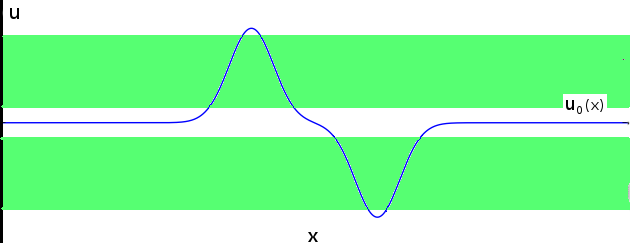
\includegraphics[height=3.3cm]{demo_theorem_1.png}
%        \caption{Illustration of $\mathcal{E}$ in theorem \ref{theorem: 1}, 
%                 the blue line shows $u_0(x)$. $\mathcal{E}$ is is colored green.}
%        \label{fig:demo_theorem_1}
%    \end{center}
%\end{figure}
%
%\noindent However, in realistic problems, generally $u$ has more than 1 dimensions.
%Besides, the primal model is a discretized PDE. It will be hard, if not impossible, 
%to give a close-form expression for $\mathcal{E}$. So we have to 
%determine $\mathcal{E}$ numerically. 




